\newif\ifdraft
%\drafttrue
\draftfalse

% Hauptdatei/ Steuerdatei für das gesamte Projekt
% Nehmen Sie bitte nur Änderungen an gekennzeichneten Stellen vor.
% Diese Stellen sind mit **manual** kenntlich gemacht.

% Klassenaufruf:
%
% Innerhalb der eckigen Klammern können Sie durch Komma getrennt
% nachfolgend aufgeführte Optionen in der Klasse steuern.
% Falls keine Optionen angegeben werden, verwendet der Compiler
% die mit * gekennzeichneten als Standard. Die Bedeutung entnehmen
% Sie bitte dem aus diesem Projekt generierten PDF Dokument.
%
% OPTIONEN:
% oneside* <-> twoside
% onecolumn* <-> twocolumn
% final* <-> draft
% fleqn
% rgbt* <-> flbt
% en <-> de*
% pdf* <-> nonpdf
%
% **manual**
\documentclass[oneside, onecolumn, final, rgbt, en, pdf]{MST_Latex2e_style}
%\usepackage{titlesec}
\renewcommand{\chaptername}{}
%\titleformat{\chapter}[display]{\normalfont\bfseries}{}{0pt}{\Large}
%\titleformat{\chapter}{\normalfont\huge}{\thechapter.}{20pt}{\huge\it}


% Integrierte Packages
%
% Die folgenden Packages sind bereits fix integriert:
% [latin1]{inputenc} - Deutsche Tastatur
% {graphicx}         - Grafikeinbindung
% {epsfig}           - Verwendung von eps Grafiken falls nonpdf
% {makeidx}          - automitisierte Indexerstellung
% {color}            - Verwendung von Farben im Text
% {supertabular}     - Mehrseitige Tabellen
% {rotating}         - Drehung von Objekten, Sidewaystable
% {float}            - Fixierung von Fliessumgebungen
% {textcase}         - Uppercase, etc.



% Optionale Usepackages
%
% Die folgenden Packages wurden hinzugefügt,
% da diese oft Verwendung finden. Diese können jedoch
% mit einem Kommentarzeichen ausgeschaltet werden, da
% User diese u.U. nicht benötigen.
%
% **manual**
\usepackage{layout}             % graphische Darstellung der Abmessungen im Kapitel Abmessungen
                                % das usepackage layout kann für die wissenschaftliche Arbeit
                                % entfernt werden
%
\usepackage{booktabs}           % Besondere Tabellenumgebung wie man sie oft im modernen
                                % Buchdruck findet
%
\usepackage[plainpages=false,pdftex,bookmarks,bookmarksopen,bookmarksnumbered]{hyperref} % colorlinks
                                % Hyperref erzeugt selbständig und mit Hilfe von Steuerbefehlen im
                                % Text ein verlinktes PDF
%
%   \usepackage{flafter}        % flafter = float after -> Kein Gleitobjekt vor Einbindungsstelle
%
%   \usepackage{amsmath}        % Erleichter die verbesserte Ausgabe bei der Verwendung mathematischer
                                %  Formulierungen in Texten; z.B. ist split eine schöne Hilfe zur Darstellung
                                % mehrzeiliger Formeln ohne eqnarray.
%
%   \usepackage{longtable}      % Tabellen können sich über Seiten fortsetzen, ohne besonderes
                                % Einwirken durch den Benutzer, ähnlich wie supertabular.
                                % Supertabular hat jedoch das umfangreichere Funktionsspektrum.
%
%
%
% User Usepackages
%
% Fügen Sie nachfolgend von Ihnen benötigte Usepackes ein.
% \usepackage[option]{packagename}
%
% **manual**
%
%
\usepackage{pdfpages}						% Für das Einbinden von mehrseitige pdf-Dateien

\usepackage{rotating}						% Für das Rotieren von Tabellen

\usepackage[bf, it, textfont=it, hang]{caption}		% Um das 'Caption' zu personalisieren

\usepackage{makeidx}
\makeindex
% 

%\usepackage[latin1]{inputenc}
%\usepackage[T1]{fontenc}
\usepackage[english]{babel}
%\usepackage[british]{babel}
\usepackage[scaled]{uarial}
\usepackage{todonotes}
\usepackage{xcolor}
\usepackage[percent]{overpic}
\usepackage{amsmath}
\usepackage{siunitx}
\usepackage{amssymb}
\usepackage[super]{nth}
\usepackage[nodayofweek]{datetime}
%\longdate
\def\today{\ifcase\month\or
  January\or February\or March\or April\or May\or June\or
  July\or August\or September\or October\or November\or December\fi
  \space\nth{\number\day}, \number\year}
%----------------------------------------------------------------
% DOKUMENT ANFANG
\begin{document}
\pagenumbering{Alph}

%  TITELSEITE EINBINDEN
% +++++++++++++++++++++++++++++++++++++++++++++++

%
% ########################################################
% TITEL-SEITE
%
% =======================================================
% (1) W�hlen Sie die Art Ihrer Abschlu�arbeit: nichtzutreffendes auskommentieren
% (2) Setzen Sie in \title den Titel Ihrer Abschlu�arbeit ein.
% (3) Ersetzen Sie " Autor durch Ihren Namen"
% (4) Setzen Sie das gew�nschte Datum, oder verwenden das auto - Datum
% (5) Geben Sie Ihre(n) Hochschulbetreuer an.
% =======================================================
%
%   (1)

%\Master

%Bachelorarbeit
%\Bachelor

%Diplomarbeit
%\Diplom

%Studienarbeit
%\Stud

%Hauptseminar
%\Hsem

%Projektpraktikum
%\Ppra

%Forschungspraxis
\Forpraxis

%Ingenieurspraxis
%\Ingpraxis

%   (2)
\title{Verification and Testing of Extended Kalman Filter for the Attitude Determination and Control System for the CubeSat MOVE-II}
%   (3)
\author{Martin Mostad}
%
%   (4)
%\date{\scalebox{.9}[.95]{26. September 2014}}
\date{\today}
%
%   (5)
\Betreuer{ Dr.-Ing. Markus Plattner}
%
% =======================================================
% Die Verwendung von thanks wird durch die Klasse unterbunden.
% Verwenden Sie stattdessen\textbf{} die Vorwort-Umgebung
% =======================================================
%
\maketitle  % !! NICHT VER�NDERN !!
% =======================================================
% Der MST Kopf erscheint nicht im DVI!!
% Es ist eine �bersetzung nach pdf notwendig!
% =======================================================
% ENDE TITEL-SEITE
% ########################################################

\pagenumbering{Roman}
%
% ZUSAMMENFASSUNG EINBINDEN
% +++++++++++++++++++++++++++++++++++++++++++++++
% Kurzfassung in Deutsch oder Englisch, maximal 650 Zeichen inkl. Leerzeichen
\begin{abstract}

Kurzfassung in Deutsch oder Englisch, maximal 650 Zeichen inkl. Leerzeichen

\end{abstract}
 
%
%
% VORWORT: FÜR VORHERGEHENDE ERLÄUTERUNGEN UND EVTL. DANKWORTE
% +++++++++++++++++++++++++++++++++++++++++++++++
% Ab hier ist die Umgebung optional und dem entsprechenden Bedürfnis angepaßt einzusetzen!
% Falls die Umgebung nicht benötigt wird, entweder mit einem Kommentarzeichen deaktivieren,
% oder den Input löschen.
%
% **manual**
%\input{Vorwort}
%
%
% INHALTSVERZEICHNIS
% +++++++++++++++++++++++++++++++++++++++++++++++
\tableofcontents
%
%
% EINLEITUNG EINBINDEN
% +++++++++++++++++++++++++++++++++++++++++++++++
%\setcounter{page}{1}%
\chapter{Introduction}

\section{CubeSat}
A CubSat is a satellite that follows the CubSat standard. The standard was initial developed in a collaboration between  California Polytechnic State University and Stanford University with the goal of giving the scientific community affordable aces to space. 

It achieves this by enforcing a strict form factor on the satellite. This gives several advantages one is that it allows for mas production of components as everybody follows the same standard. It also means that the process of finding a launch provider is a lot easier. As they all have the same form factor standardized launch interfaces have been created and even the ISS have the opportunity to launch CubSat. 

The most important part of the specification is the size and weight. CubeSats can come in different size but they are all based on the 'unit' called 1U. A 1U is 10x10x10cm cube that can weigh no more than 1.33 kg. You can get different sizes by staking 1Us together. Normal sizes are 1U, 2U,3U and 6U. The limit in size and weight heavily influences the design and means you very often are working with limited battery capacity. It also affect the ADCS system as it becomes difficult to add truster and adding reaction wheels become a big cost as they take a lot of space and weight\cite{CubeSat101}.                         

\section{The MOVE-II CubeSat}
The MOVE-II CubeSat is a 1U CubeSat. It is a project at the Lehrstuhls f�r Raumfahrttechnik(LRT) whit support from Deutsche Luft- und Raumfahrtzentrum(DLR) and in cooperation with the Wissenschaftlichen Arbeeitsgemenschaft f�r Raketentechnik und Raumfahrt(WARR). 


\ifdraft
The MOVE-II CubeSat consists primarily of seven subsystems. 

\subsubsection{Thermal}
The Thermal subsystem is in charge of monitoring the temperature of satellite and make sure that it does not overheat. It was also a big part in the design to make sure there where no parts that is designed in such a way that they produce to much heat. 

\subsubsection{Communication}
The communication subsystem has the responsibility of the radio communication between the satellite a and the ground station. The satellite is equipped with a UHF/VHF antenna and and S-Band antenna. 

\subsubsection{Computer data handler}
works as the main      
\fi

Most of the students working on the project are volunteers. As the development face of the project is ending whit the planed launch in October the number of active students is going down but at the most there was over a 100 students working on the project. There is still a lot of work that can be done on the project, even if the satellite is launching in October. Both in therms of data analysis and future development of software as most of the software can be updated once the satellite is in orbit. 

This is especially true for the ADCS as it generates a lot of sensor data and there are many parts of the software that can be improved. One of these improvements for the ADCS is to activate the extended kalam filter(EKF). The EKF was not sufficiently tested before the launch software was frozen so it is not a part of the launch. At a later time and as a part of this rapport significant effort has been put into testing the EKF so it can be implemented as soon as the projects open up for uploading new software to the satellite.               

\section{Altitude determination and control system}
The altitude determination and control system (ADCS) of a satellite has the task of determining and controlling the altitude of the satellite. For the MOVE-II mission it is required that the top panel of the satellite is pointing towards the sun. This is has two reasons. The first is that the payload requires sun pointing. The experimental solar cells positioned on the top panel require to be in the sun so their efficiency can be measured. The second reason is that the satellite has four flap panels that will be deployed after launch to a position where they creates a large area of solar cells with the top panel see figure \ref{fig:Sat_Deployed}. So to maximize this solar cells they should be facing the sun.

\begin{figure}[tbp]
	\centering
	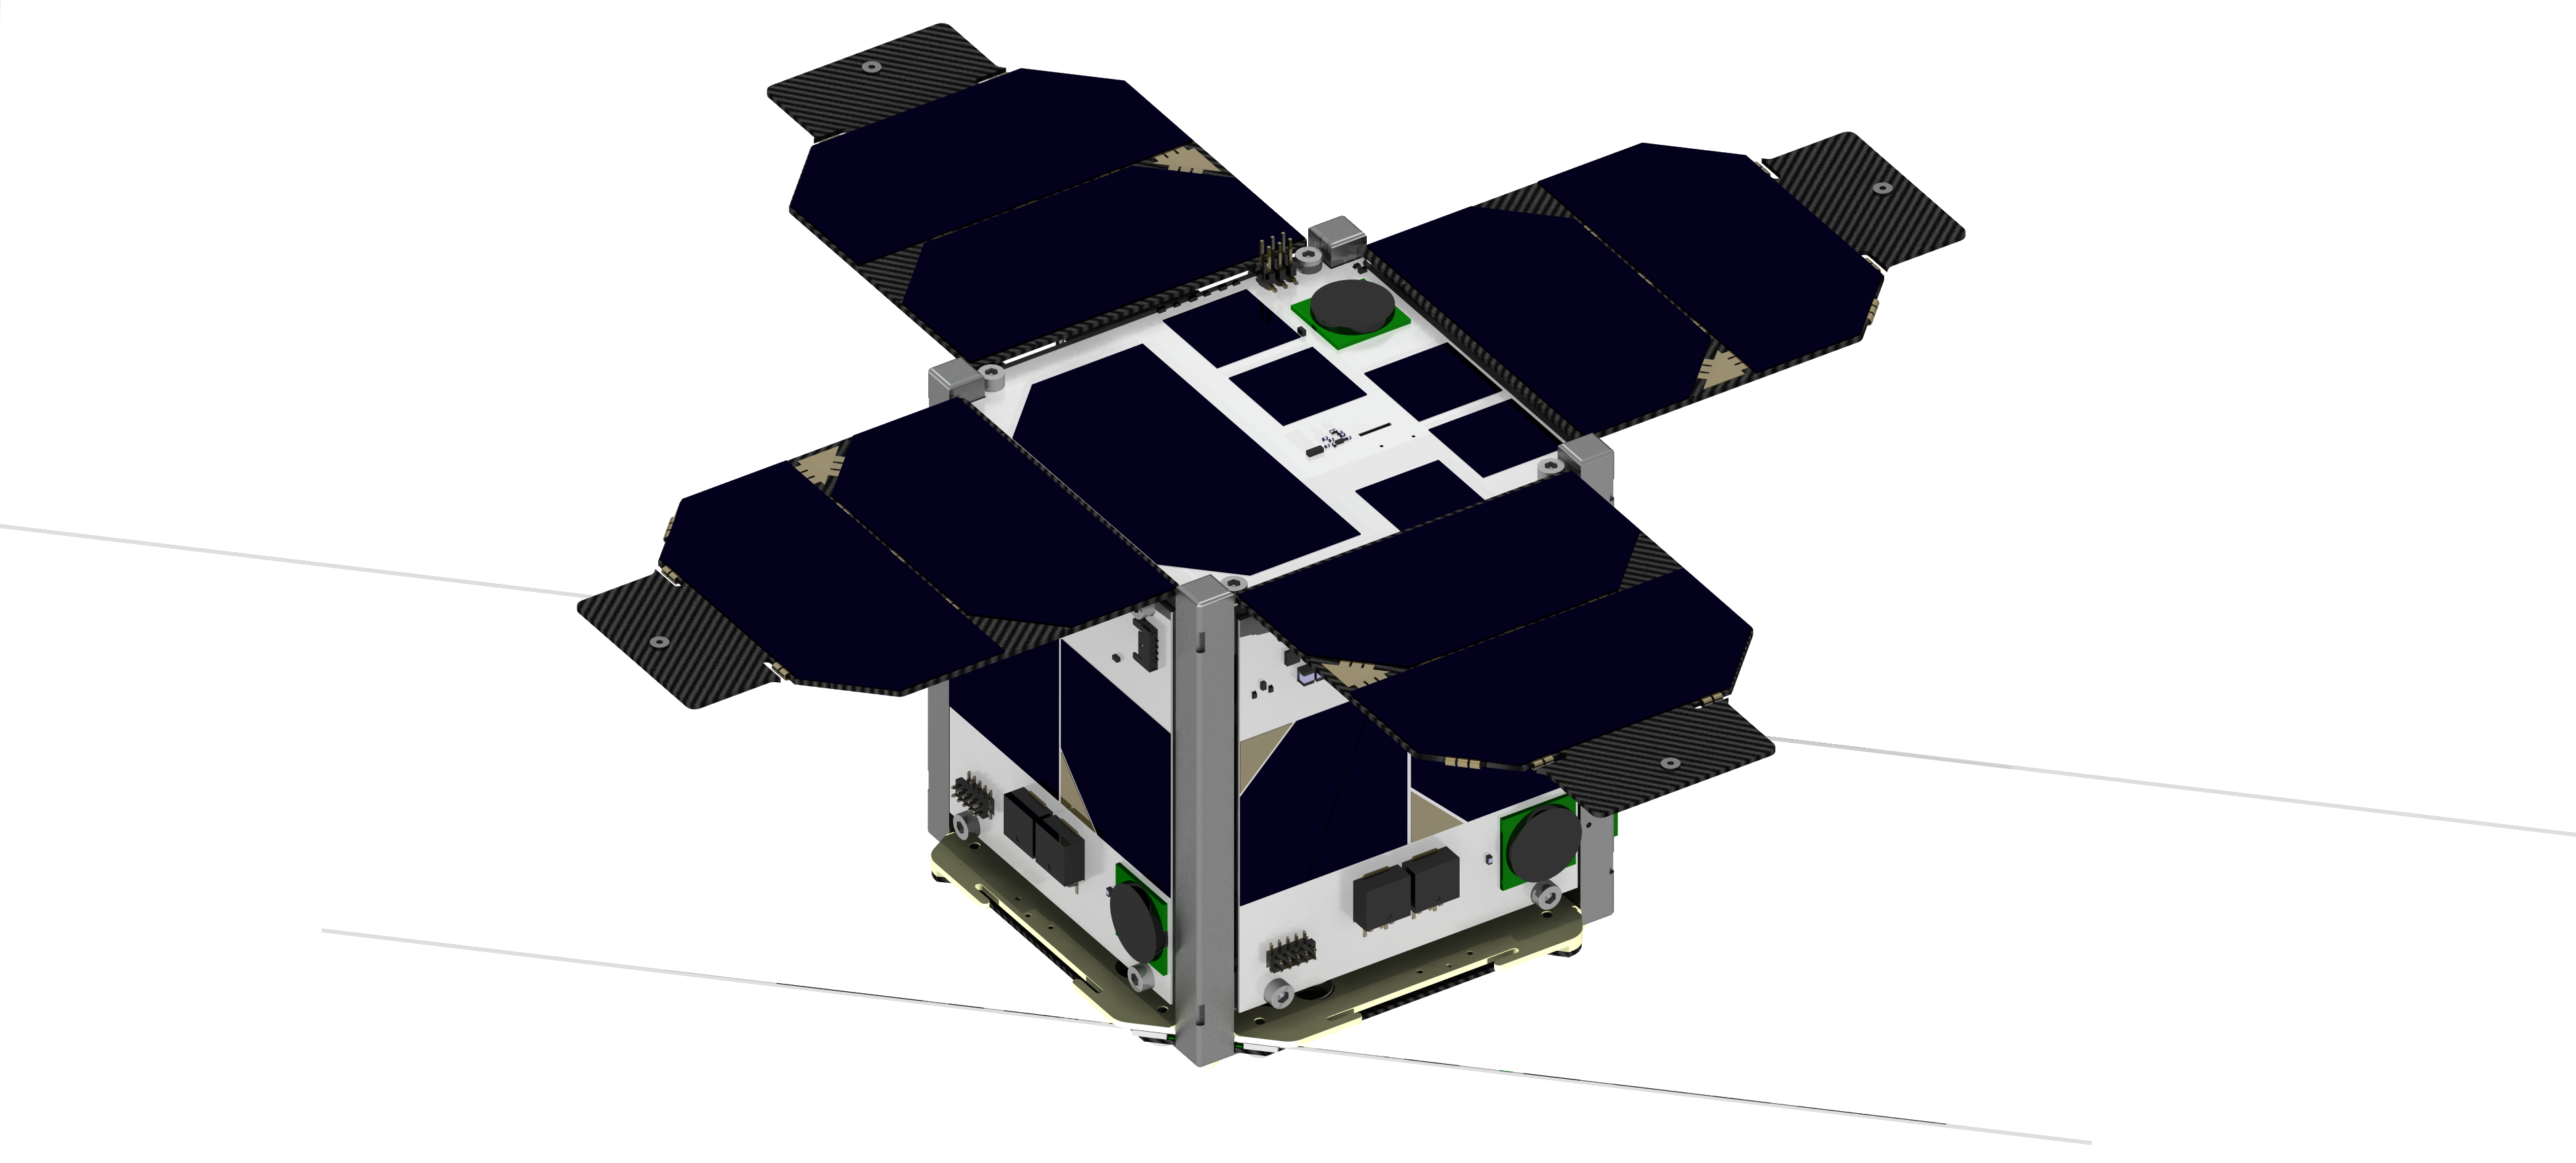
\includegraphics[width=\linewidth,scale=1]{./Pictures/SatelliteDeployed}
	\caption{Rendering of the MOVE-II CubeSat with flap panels deployed}
	\label{fig:Sat_Deployed}
\end{figure}

The ADCS is normally a complex system that can be designed in many different ways. In general on a high level the ADCS can be described as a classical control system consisting of a control component, actuator component and sensor component creating a closed loop control system. There might also be observers or estimators either to use the estimates in the controller or for simply recording the estimated position of the satellite. The normal actuators for satellites are coils interacting with the magnetic felled of the earth to create a torque see equation \ref{eq:Mag_Control} \cite{move-ii-sysdoc}, reaction whiles or thrusters. For the CubSats the most common is magnetic coils and sometimes reaction whiles. Thrusters are very rarely used. The sensor can consists of many different sensors and it is very common to combine several types of sensors. Common sensors include magnetometers to measure the magnetic felled of the earth. Light sensors often named sun sensors that measure light intensities and can be used to determine the direction of the sun. Gyroscopes to measure the rotation of the satellite. If estimators are used the sensor data is very often used in combination with models of the sun position like the SG4 and models of the magnetic felled like IGRF.                    

\begin{equation}\label{eq:Mag_Control}
	\vec{T} = \vec{M} x \vec{B}
\end{equation}

\subsection{MOVE-II ADCS architecture}
The adcs system for MOVE-II consists of six panels see figure .. for placement in satellite. Each having a microcontroller, BMX sensor, coils and a sun sensor except for the main panel that does not have a sun sensor. The BMX sensor is a combined accelerometer, gyroscope, magnetometer and temperature sensor. The task of the microcontrollers that are not on the main panel is mainly to collect sensor data and control their respective coils. The microcontroller on the main panel also collects sensor data and controls it`s coils. In addition it is ruining the control algorithm, EKF, all the models that are required for the EKF and it communicates with the rest of the satellite. The main panel gets all the sensor data from the rest of the panels and biased on this the control algorithm calculates the appropriate current for each panel that it sent back to all the other microcontrollers.

\begin{figure}[tbp]
%	\centering
	\begin{overpic}[]{./Pictures/ADCSPanelOverwive}
	\put(30,50){\color{black}\rule{1pt}{30pt}}
	\caption{The placement and name of the different panel of the ADCS}
	\label{fig:Sat_Deployed}
\end{figure}

The ADCS has 4 modes; SLEEP, ATTDET, DETUMBL and SUN. In SLEEP the ADCS does not control anything and is only recording minimal sensor data. The ATTDET mode the ADCS calculates the attitude of the satellite with a frequency of ... it does not do any controlling. In the DETUMBL mod the goal is to detumble the satellite down to ... This mode if intended to be used after the satellite is released from the pod as it is expected to have a high velocity of ... . For this purpose the ADCS uses a bdot controller. The control law can be seen in eq ... . In the SUN mode the ADCS tries to point the top panel towards the sun. For this a spinning controller is used with a velocity of 5.7 deg/s. The control law can be seen in eq ... .                                         
%
%
% HAUPTTEIL EINBINDEN
% +++++++++++++++++++++++++++++++++++++++++++++++
% Die Eingebundene Datei Hauptteil sollte erhalten bleiben.
% Zum Einen können Sie dann den kompletten Hauptteil
% auf einmal auskommentieren, wenn Sie an anderen
% Teilen arbeiten. Ausserdem erhöht die Einbindung Ihrer
% Kapitel in der Datei Hauptteil.tex die Übersichtlichkeit.
% Zudem finden sich die einzelnen Einbingsstellen gut, wodurch
% sich auch einzelne Kapitel auskommentieren lassen.
%
% **************************************************************
% **************************************************************
%
% HIER SIND DIE KAPITEL DER ARBEIT IN GEEIGNETER FORM EINZUBINDEN
%
%
%\chapter{Sensor models}
\label{sensorModels}

\section{Magnetometer}
\subsection{Mathematical model}
\subsection{Calibration method}

\section{Gyroscope}
\subsection{Mathematical model}
\subsection{Calibration method}

\section{Sun sensor}
\subsection{Mathematical model}
\subsection{Calibration method}

\chapter{Attitude Determination Methods}\label{chap:EKF}

Attitude determination can be defined as finding the minimal parameterization of the attitude matrix whit the help of some measurement data. Generally speaking attitude determination methods can be divided into two categories. The first category are static methods. They relay only on measurements taken at the same time and are reliant on critical number of measurements at any given time to function. Examples of such methods are the TRIAD algorithm or solving Wahba's problem. The second category are filtering methods which uses a history of data and a dynamic model of the satellite. Examples of such models are variations of the Kalman filters \cite{SADCS}.        

\section{Attitude Determination Methods in CubeSats}
For attitude determination the extended Kalman filter (EKF) is the standard method and have a good record even if it has some problems. This problems mostly arises from the linearization that the filter performs \cite{attdetSur}. For the design of the MOVE-II attitude determination system (ADS) three other CubeSats ADS where studied \cite{DavidThesis}. 

\begin{itemize}
  \item \textbf{UWE3:} The third CubeSat of the University of Würzburg in Germany \cite{UWE-3}.
  \item \textbf{AAUSAT-3:} The third CubeSat of the Aalbord University in Denmark \cite{aausat}. 
  \item \textbf{ESTCube-1:} The first CubeSat of the University of Tartu, Estonia \cite{EST}.
\end{itemize}       

The ADS on all this systems have a lot of similarities to the ADS of MOVE-II. They are all based around the same sensors namely sun sensors, gyroscope and magnetometers. Because they have the same sensor set as the MOVE-II they also use many of the same models like the earth's magnetic field model and sun position model. In the end all this data is combined using some form of Kalman filter. They all vary slightly from each other and from the MOVE-II implementation. 

The UWE3 uses a Isotropic Kalman filter. The Isotropic Kalman filter is a recursive state estimation based on the dynamic model of the system. The state vector of the Kalman filter is the vector component of the quaternion and the bias of the gyroscope\cite{UWE-3}. The AAUSAT-3 uses a combination of an SVD-method to solve Wahba's problem and an unscented Kalman filter (UKF). Where the SVD-method is used to give a good initial estimate for the UKF. A UKF differs from a Kalman filter in that instead of using the last estimate to generate the prediction it uses a sigma point. Where a sigma point is a structured set of sampling points representing the probability distribution of the point. For a more in depth view look at \cite{attdetSur}. The ESTCube-1 also uses a UKF as their on board ADS. They also have a image-based attitude Simplified General Perturbationdetermination system that they use to verify the result of the UKF based ADS. The image-based system is done in a post processing proses on ground \cite{EST}

\section{Attitude Determination on MOVE-II}
The ADS on MOVE-II is based around an EKF that is initialized by the solution to Wahba's problem using SVD-methods. Overall structure of the ADS can be seen in \autoref{fig:ADS_overview}. There are two main parts going into the Attitude Determination Algorithms. The sensor measurements and the model output. The sensor measurements are preprocessed before they are sent to the algorithms. The models that are used will be future discussed in \autoref{subsec:ModelADS}. The SVD-method uses the model output and the sensor measurements to calculate an initial estimate for the EKF. The EKF then estimates the quaternion representing the rotation from Earth Centered Inertial frame (ECI) to the satellite body-fixed frame. The ECI is defined similarly to what is called the Geocentric Inertial Frame in \cite{SADCS}. Where the origin of the frame is at the center of mass of the earth. The z-axis is aligned with the earth's north pole. The x-axis is directed towards the vernal equinox. The vernal equinox the intersection of the earth's orbital plane and the earth's equatorial plane. The y-axis is defined to complete the coordinate frame with the right hand rule. The body-fixed frame is defined as having its origin at the center of mass of the satellite and the axis are parallel to the panels of the satellite. The z-axis is defined to point away from the top panel as shown in figure \autoref{fig:bodyFix}. The EKF also outputs an bias compensated angular velocity based on an estimate of the bias on the gyroscopes.

\begin{figure}[tbp]
	\centering
	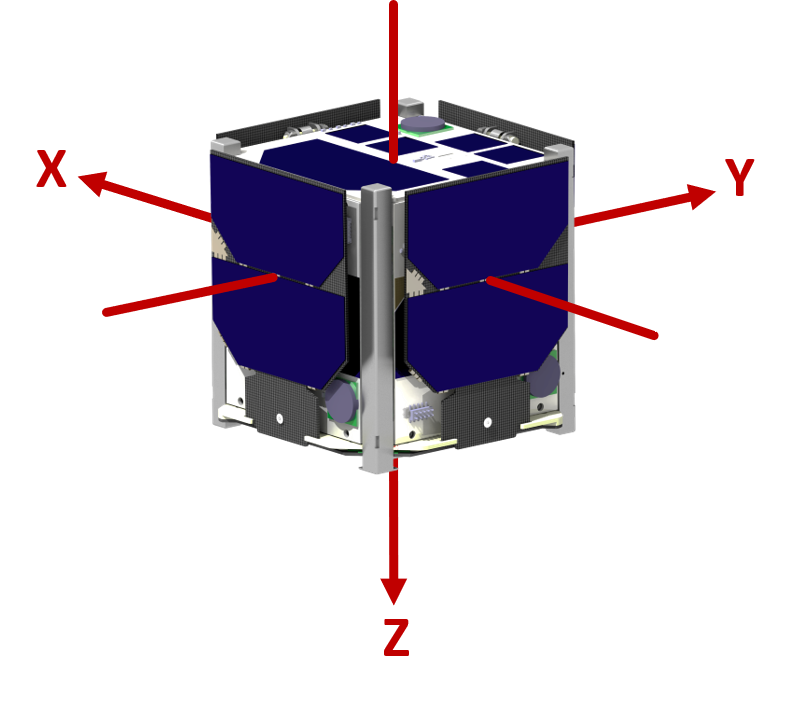
\includegraphics[width=0.6\columnwidth]{./Pictures/GBF_new}
	\caption{The body-fixed frame drawn on the satellite from \cite{DavidThesis}}
	\label{fig:bodyFix}
\end{figure} 

\begin{figure}[tbp]
	\centering
	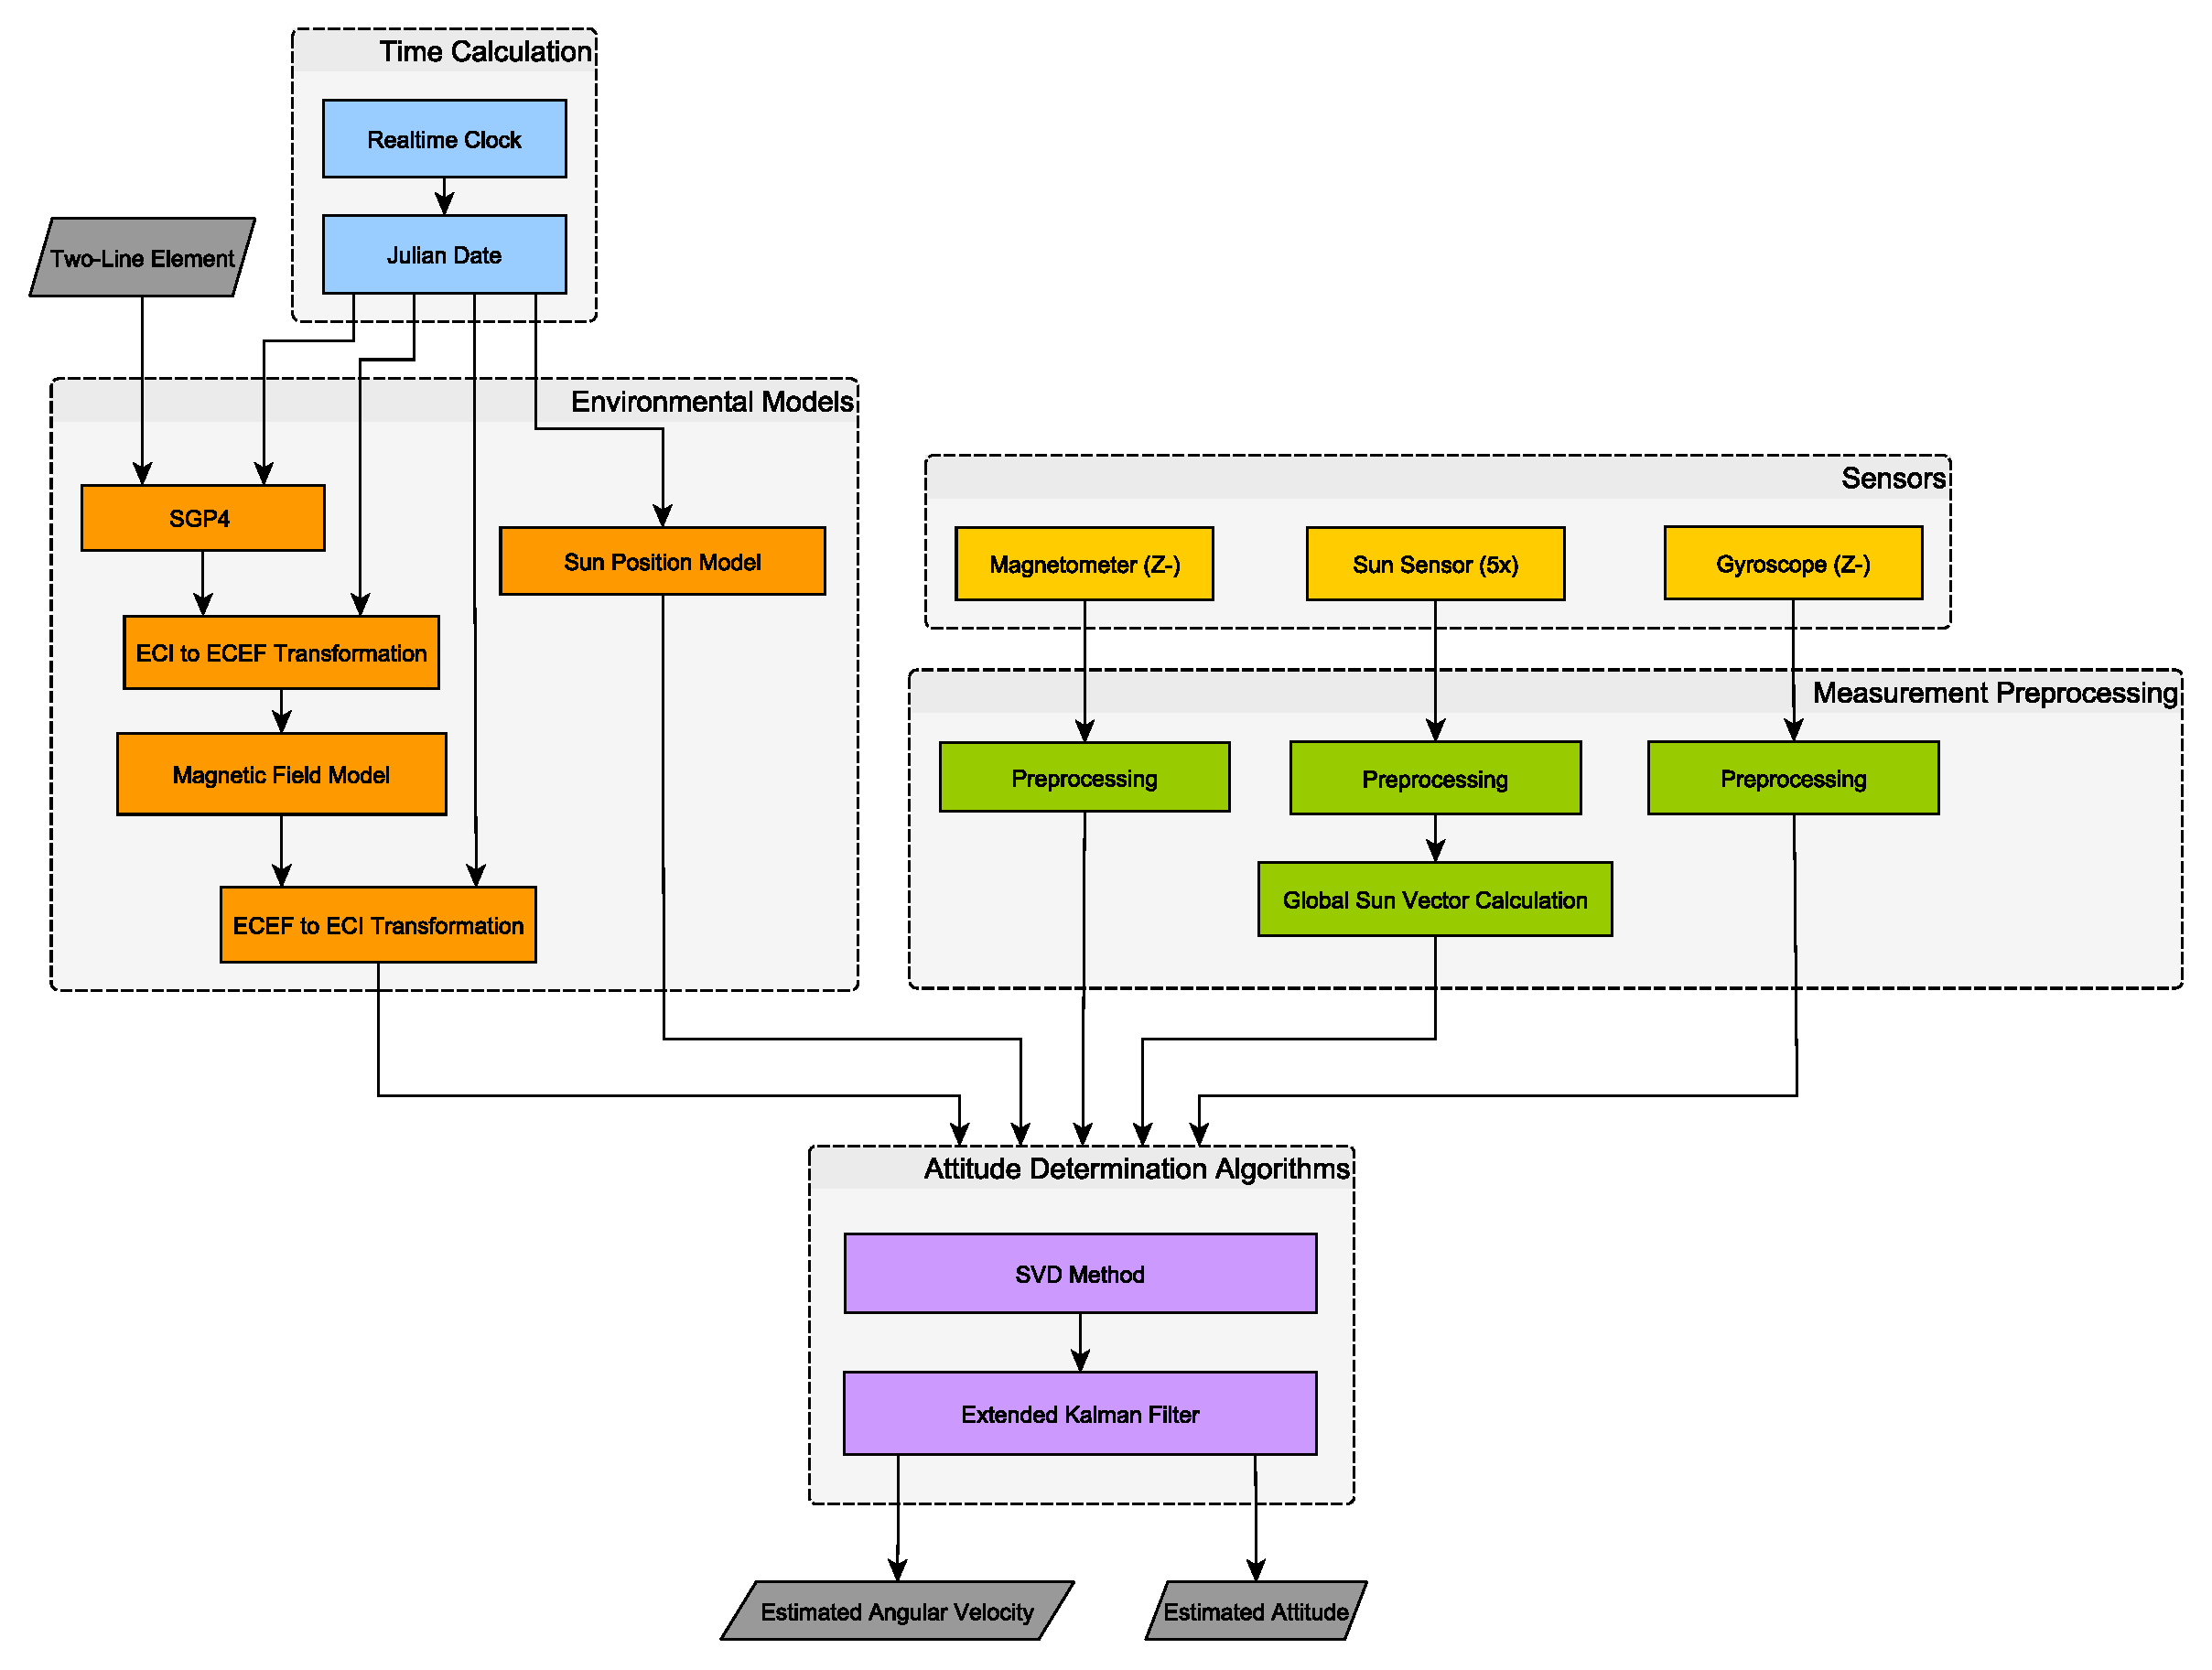
\includegraphics[width=0.5\columnwidth]{./Pictures/ATTDET_Architecture_new}
	\caption{Overview of the submodules that make up the complete Attitude Determination Systems from \cite{DavidThesis}}
	\label{fig:ADS_overview}
\end{figure}            

\subsection{Models Used in Attitude Determination}\label{subsec:ModelADS}
There are two main models used in the ADS. It is sun position model and a model of the earth's magnetic field. The output from both of this models are normalized vectors resolved in the ECI frame. The vectors will be used as reference vectors in both the SVD and the EKF. 

The sun model is the one described in \cite{AstroPC}. The sun model requires the Julian Date. The Julian Data is calculated from the real time clock that is part of the ADCS. The clock can also be resynchronized to the system time of the satellite \cite{DavidThesis}. 

The model of the earth's magnetic filed is the International Geomagnetic Reference Model (IGRF)\cite{IGRF}. The IGRF needs the orbit position as an input. To get the orbit the Simplified General Perturbation Model 4 (SGP4) is used, it is described in more detail in \cite{SGM4}. This model requires a Two Line Element (TLE) and the Julian Data to function. The IGRF needs the position of the satellite in Earth Centered Earth Fixed (ECEF) frame and to outputs the magnetic field vector in ECEF frame. Where ECEF is defined as origin at earth's center of mass. Z-axis aligned with the north pole, x-axis pointing towards the intersection between Earth's primary meridian and equator and the y-axis is defined to complete the coordinate frame according to the right hand rule. To accommodate this change in coordinates a function to generate the rotation matrix to go from ECI to ECEF frame was needed. This function is time dependent as the ECEF frame rotates in the ECI frame. The implementation of the SGI4, the IGRF and the function to find the rotation from ECI to ECEF frame are all based on the work in \cite{aausatMasterThisis} as stated by \cite{DavidThesis}. 

\subsection{SVD-Method to Solve Wahba's problem}
Wahba's problem is the least square optimization problem where you have a to minimize the cost function $J(A)$ show in \autoref{eq:Wahba'sProblem}. Where $b_i$ and $r_i$ are the same observations redissolved in two different frames. $A$ is an orthogonal matrix representing the rotation from the frame of $r_i$ to $b_i$ \cite{aausat}. So if $b_i$ are the observations from the models in ECI and $r_i$ are the sensor measurements in the body-fixed frame then by solving Wahba's problem you will get the rotation matrix from body-fixed frame to ECI.     

\begin{equation}\label{eq:Wahba'sProblem}
	J(A) = \sum\limits_{i=1}^{m}a_i||b_i - Ar_i||^2
\end{equation}

The cost function can be reformulated to \autoref{eq:Wahba'sProblemReformul} \cite{aausat}. Where $B = \sum\limits_{i=1}^{m}a_ib_ir_i^T$. It is clear now that this reduces Wahba's problem to maximizing $trace(AB^T)$, where the SVD-method is a fast and robust algorithm to solve this problem. For a more rigorous deduction of the algorithm see \cite{DavidThesis} or \cite{aausat}.

\begin{equation}\label{eq:Wahba'sProblemReformul}
	J(A) = \sum\limits_{i=1}^{m}a_i - trace(AB^T)
\end{equation}

\subsection{Extended Kalman Filter on MOVE-II}\label{chap:EKF_MOVE_II}
The full EKF will not be fully explained or derived in this report. Instead the key features and implementations will be highlighted. For a more in depth view into EKF see \cite{DavidThesis} or \cite{indirectKalman} which is the derivation followed here.  

The EKF that is used on the MOVE-II satellite is not based on the dynamic model of the satellite, but rather uses the gyroscope measurements directly in the models. Rather than using it as a measurement. This means that the gyroscope measurements replaces the dynamic model. This has two main advantages. The first is that the gyroscope measurements might be more accurate than the dynamic model. The second is that this method is a lot less computational expensive. To use the gyroscope measurements to replace dynamic model a model of the gyroscopes is instead needed. The gyroscope can be modeled as shown in \autoref{eq:gyroModel}. Where $\tilde{\boldsymbol{\omega}} \in \mathbb{R}^{3}$ is the measured angular velocity from the gyroscope and $\boldsymbol{\omega} \in \mathbb{R}^{3}$ is the true angular velocity. $\boldsymbol{\beta} \in \mathbb{R}^{3}$ is the bias of the gyroscope modeled as a random walk. $\boldsymbol{\eta_v} \in \mathbb{R}^{3}$ and $\boldsymbol{\eta_u} \in \mathbb{R}^{3}$ are independent Gaussian with white noise with zero mean.               

\begin{align}
	\tilde{\boldsymbol{\omega}} &= \boldsymbol{\omega} + \boldsymbol{\beta} + \boldsymbol{\eta_v}\label{eq:gyroModel}\\
	\dot{\boldsymbol{\beta}} &= \boldsymbol{\eta_u}\label{eq:randomWalk} 
\end{align}

The state vector for the EKF is defined as $\boldsymbol{x} \in \mathbb{R}^{7}$ consisting of the rotation quaternion representing the rotation between body-fixed frame and ECI frame $q \in \mathbb{R}^{4}$ and the gyroscope bias $\boldsymbol{\beta} \in \mathbb{R}^{3}$.

\begin{equation}\label{eq:stateVectorEKF}
	\boldsymbol{x} = \begin{bmatrix}
    		\boldsymbol{q} \\ \boldsymbol{\beta} & 
		 \end{bmatrix}\\
\end{equation}

Given the gyroscopic \autoref{eq:gyroModel} a system of differential equation for the states can be written as \autoref{eq:diffEq}  
\begin{subequations}\label{eq:diffEq}
\begin{align}
	\boldsymbol{\dot{q}} &= \frac{1}{2}\boldsymbol{\Omega}(\tilde{\boldsymbol{\omega}} - \boldsymbol{\beta} - \boldsymbol{\eta_v})\boldsymbol{q}\label{eq:diffQuaternion}\\
	\boldsymbol{\dot{\beta}} &= \boldsymbol{\eta_u}
\end{align} 
\end{subequations}

Where $\boldsymbol{\Omega}$ is defined in \autoref{eq:omega} and $[\cdot\times]$ is defined as skew-symmetric operation. 

\begin{equation}\label{eq:omega}
	\boldsymbol{\Omega}(\boldsymbol{\omega}) = \begin{bmatrix}
		-[\boldsymbol{\omega}\times]^T & \boldsymbol{\omega} \\
		-\boldsymbol{\omega}^T & 0 \\ 
		\end{bmatrix}
\end{equation} 

This leads to the propagation equation shown in \autoref{eq:propagation} at time k. Where $\hat{\cdot}$ is an estimate, + means the corrected estimate and - is the output from the propagation step. 

\begin{subequations}\label{eq:propagation}
\begin{align}
	\hat{\boldsymbol{\beta}}^-_k &= \hat{\boldsymbol{\beta}}^+_{k-1} \\
	\hat{\boldsymbol{\omega}}^-_k &= \tilde{\boldsymbol{\omega}}_k-\hat{\boldsymbol{\beta}}^+_{k-1} \\
	\hat{\boldsymbol{q}}^-_k &= (\boldsymbol{I}_{4\times4} + \frac{\Delta t}{2}\boldsymbol{\Omega}(\hat{\boldsymbol{\omega}}^+_{k-1}))\hat{\boldsymbol{q}}^+_{k-1}
\end{align}
\end{subequations}

For the update step the measurement vector $\boldsymbol{z}_k \in \mathbb{R}^{6}$ is defined as in \autoref{eq:measurment}. Where $\tilde{\boldsymbol{b}}_k \in \mathbb{R}^{3}$ is the measured magnetic vector and $\tilde{\boldsymbol{s}} \in \mathbb{R}^{3}$ is the measured sun vector at time $k$. 

\begin{equation}\label{eq:measurment}
	\boldsymbol{z}_k = \begin{bmatrix}
		\tilde{\boldsymbol{b}}_k \\
		\tilde{\boldsymbol{s}}_k \\
	\end{bmatrix}
\end{equation}  

The estimated measurement vector $\boldsymbol{h}_k \in \mathbb{R}^{6}$ is defined as in \autoref{eq:estimatedMeasurment}. Where $\boldsymbol{A}(\hat{\boldsymbol{q}}^-_k)$ is the rotation matrix from ECI frame to body-fixed frame based on the current uncorrected estimate of the quaternion $\hat{\boldsymbol{q}}^-_k$. $\boldsymbol{r}_{mag} \in \mathbb{R}^{3}$ is the reference vector for the magnetic field based on the IGRF model and $\boldsymbol{r}_{sun} \in \mathbb{R}^{3}$ is the reference vector from the sun position model. This means that $\boldsymbol{h}_k$ is the reference vectors resolved in the body-fixed frame.   

\begin{equation}\label{eq:estimatedMeasurment}
	\boldsymbol{h}_k = \begin{bmatrix}
		\boldsymbol{A}(\hat{\boldsymbol{q}}^-_k)\boldsymbol{r}_{mag} \\
		\boldsymbol{A}(\hat{\boldsymbol{q}}^-_k)\boldsymbol{r}_{sun} \\
	\end{bmatrix}
\end{equation}

The error vector $\boldsymbol{\epsilon}_k \in \mathbb{R}^{6}$ is then defined as the difference between the measurement vector $\boldsymbol{z}_k$ and the estimated measurement vector $\boldsymbol{h}_k$, as shown in \autoref{eq:errorVector}. 

\begin{equation}\label{eq:errorVector}
	\boldsymbol{\epsilon}_k = \boldsymbol{z}_k - \boldsymbol{h}_k
\end{equation}  

For the correction step the estimate of the error state vector $\delta\hat{\boldsymbol{x}}_k \in \mathbb{R}^{6}$ shown in \autoref{eq:errorStateVector}.       

\begin{equation}\label{eq:errorStateVector}
	\delta\hat{\boldsymbol{x}}_k = \begin{bmatrix}
		\delta\hat{\boldsymbol{\vartheta}}_k \\
		\delta\hat{\boldsymbol{\beta}}_k \\
	\end{bmatrix}
\end{equation} 

Where the relations between $\delta\hat{\boldsymbol{\vartheta}}_k$ and $\delta\hat{\boldsymbol{q}}^+_k$ is shown in \autoref{eq:stateRelation}.

\begin{equation}\label{eq:stateRelation}
	\delta\hat{\boldsymbol{q}}^+_k = \frac{1}{\sqrt{1- ||\delta\hat{\boldsymbol{\vartheta}}_k||^2/4}}\begin{bmatrix}
			\delta\hat{\boldsymbol{\vartheta}}_k/2 \\
			1 \\
		\end{bmatrix}
\end{equation}

$\delta\hat{\boldsymbol{q}}^+_k$ represent the error between the true quaternion and the estimated one. It is represented as the rotation between the true quaternion and the estimated quaternion instead of as a simple arithmetic as this leads to numerical issues \cite{DavidThesis}. It is defined by \autoref{eq:errorQuaternion}. $\delta\hat{\boldsymbol{\beta}}_k$ is simply defined as the difference between the true bias and the estimated bias as shown in \autoref{eq:errorBias}.

\begin{subequations}
\begin{align}
	\boldsymbol{q} &= \delta\boldsymbol{q}\otimes\hat{\boldsymbol{q}}\label{eq:errorQuaternion} \\
	\delta\boldsymbol{\beta} &= \boldsymbol{\beta} - \hat{\boldsymbol{\beta}}\label{eq:errorBias} 
\end{align}
\end{subequations} 

The error state vector $\delta\hat{\boldsymbol{x}}_k$ is calculated by \autoref{eq:calcErrorState}. Where $\boldsymbol{K}$ is the Kalman gain. 

\begin{equation}\label{eq:calcErrorState}
	\delta\hat{\boldsymbol{x}}_k = \boldsymbol{K}\boldsymbol{\epsilon}_k
\end{equation}

This finely leads to the correction step show in \autoref{eq:correctionStep}. 

\begin{subequations}\label{eq:correctionStep}
\begin{align}
	\hat{\boldsymbol{q}}^+_k &= \delta\hat{\boldsymbol{q}}^+_k\otimes\hat{\boldsymbol{q}}^-_k \\
	\hat{\boldsymbol{\beta}} &= \hat{\boldsymbol{\beta}}^-_k + \delta\hat{\boldsymbol{\beta}}^+_k 
\end{align}
\end{subequations} 


\chapter{Tests}\label{chap:tests}
Testing of an ADS is challenging as it is difficult to replicate the space environment on Earth. Therefore a lot of testing of ADS relay heavily on simulations. Simulation on the other hand have their own problems as there is a limit on how accurate they can be and they will never truly repentance the system they are simulating. In this chapter the different methods and work flow that was used for testing the MOVE-II ADS will be presented. There will be a special focus on the full hardware tests. For a more in depth view of the simulation based methods see \cite{DavidThesis}           

\section{Test Methods}
In general there where four main categories of test conducted to test and verify the MOVE-II ADS. The tests vary in there use of simulations from completely dependent on simulations to using no simulation. 

\begin{itemize}
  \item \textbf{Simulation-only:} The entire ADS is simulated along with all required environmental models, dynamic models and sensor models. Used for tuning of the Kalman filter and as a baseline check for all other tests.   
  \item \textbf{Software-in-the-Loop:} The ADS is implemented in code as it is on the satellite. The ADS is then given data generated by the simulation environment. Allows for good testing of the code to make sure it is implemented in a way that is consistent with the simulated implementation.    
  \item \textbf{Hardware-in-the-Loop:} The ADS code is running on the same micro-controller that is used on the satellite. It still gets sensor data from the simulated environment. Used to check for numerical issues on the micro-controller and to look for issues regarding timing on the micro-controller. The system is now running in real time.    
  \item \textbf{Hardware-only:} The complete ADS is tested. Where real sensor data is used by the micro-controller. The downside is that the sensor data does not necessarily represent how the sensor data would look in space as the sensors are not in space. Test the complete system and specifically how the algorithms handle real sensor data.        
\end{itemize}  

In \autoref{fig:workFlow} you can see how the different categories influence each other. An important point is how the different test categories influence each other. Where all the test categories are uses the results from the other categories as a reality check and to specify exactly what kind of scenarios should be tested. The figure also shows how dependent all the test are on good characterization and understanding of how the sensors work. 

\begin{figure}[tbp]
	\centering
	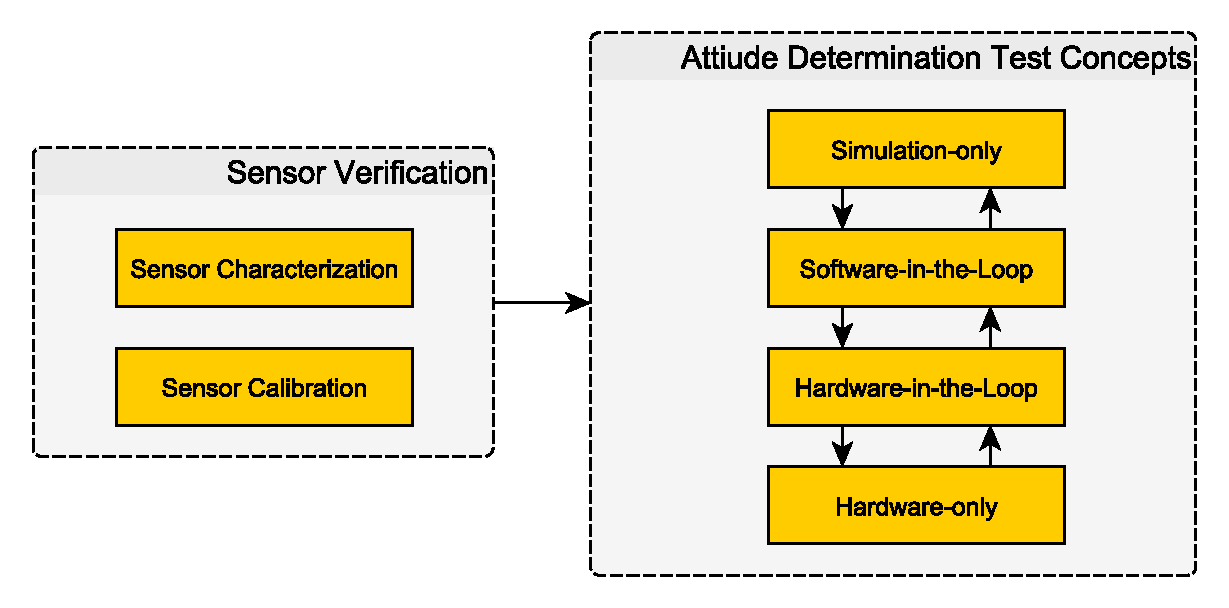
\includegraphics[width=0.7\columnwidth]{./Pictures/testing_concept}
	\caption{Relationshipp between test categories and sensor verification from \cite{DavidThesis}.}
	\label{fig:workFlow}
\end{figure}            

\subsection{Hardware-only}\label{chap:HardwareOnly}
For the Hardware-only test there were four different test cases that were considered, but ultimately only two of them were chosen do there difficulty in execution. All four will be presented before the chosen two will be described in more detail. The two chosen methods where the Algorithm Only approach and the Outdoor test approach.   

\paragraph{Algorithm Only}
The Algorithm Only approach is based around the idea of creating a reference frame around the average of sensor measurements instead of using the reference models as described in \autoref{chap:EKF_MOVE_II}. In other words $\boldsymbol{r}_{mag}$ and $\boldsymbol{r}_{sun}$ are replaced by $\tilde{\boldsymbol{r}}_{mag}$ and $\tilde{\boldsymbol{r}}_{sun}$ respectively and they are defined as in \autoref{eq:avrgLabFrame}. Where $\boldsymbol{b}_i$ and $\boldsymbol{s}_i$ are individual magnetometer and sun sensor measurements respectively.  

\begin{subequations}\label{eq:avrgLabFrame}
\begin{align}
	\tilde{\boldsymbol{r}}_{mag} &= \frac{1}{10}\sum\limits_{i=1}^{10}\boldsymbol{b}_i \\
	\tilde{\boldsymbol{r}}_{sun} &= \frac{1}{10}\sum\limits_{i=1}^{10}\boldsymbol{s}_i 
\end{align}	
\end{subequations}  

The overview shown in \autoref{fig:ADS_overview} can then be modified to reflect this changes as shown in \autoref{fig:outdoorOverview}. The main advantage of this method is that it allows for the testing of ADS with real sensor data without the need for creating a realistic space environment as the models are not used. This method also has some history within the MOVE-II as a similar approach has been used for initial testing earlier \cite{DavidThesis}. 

\begin{figure}[tbp]
	\centering
	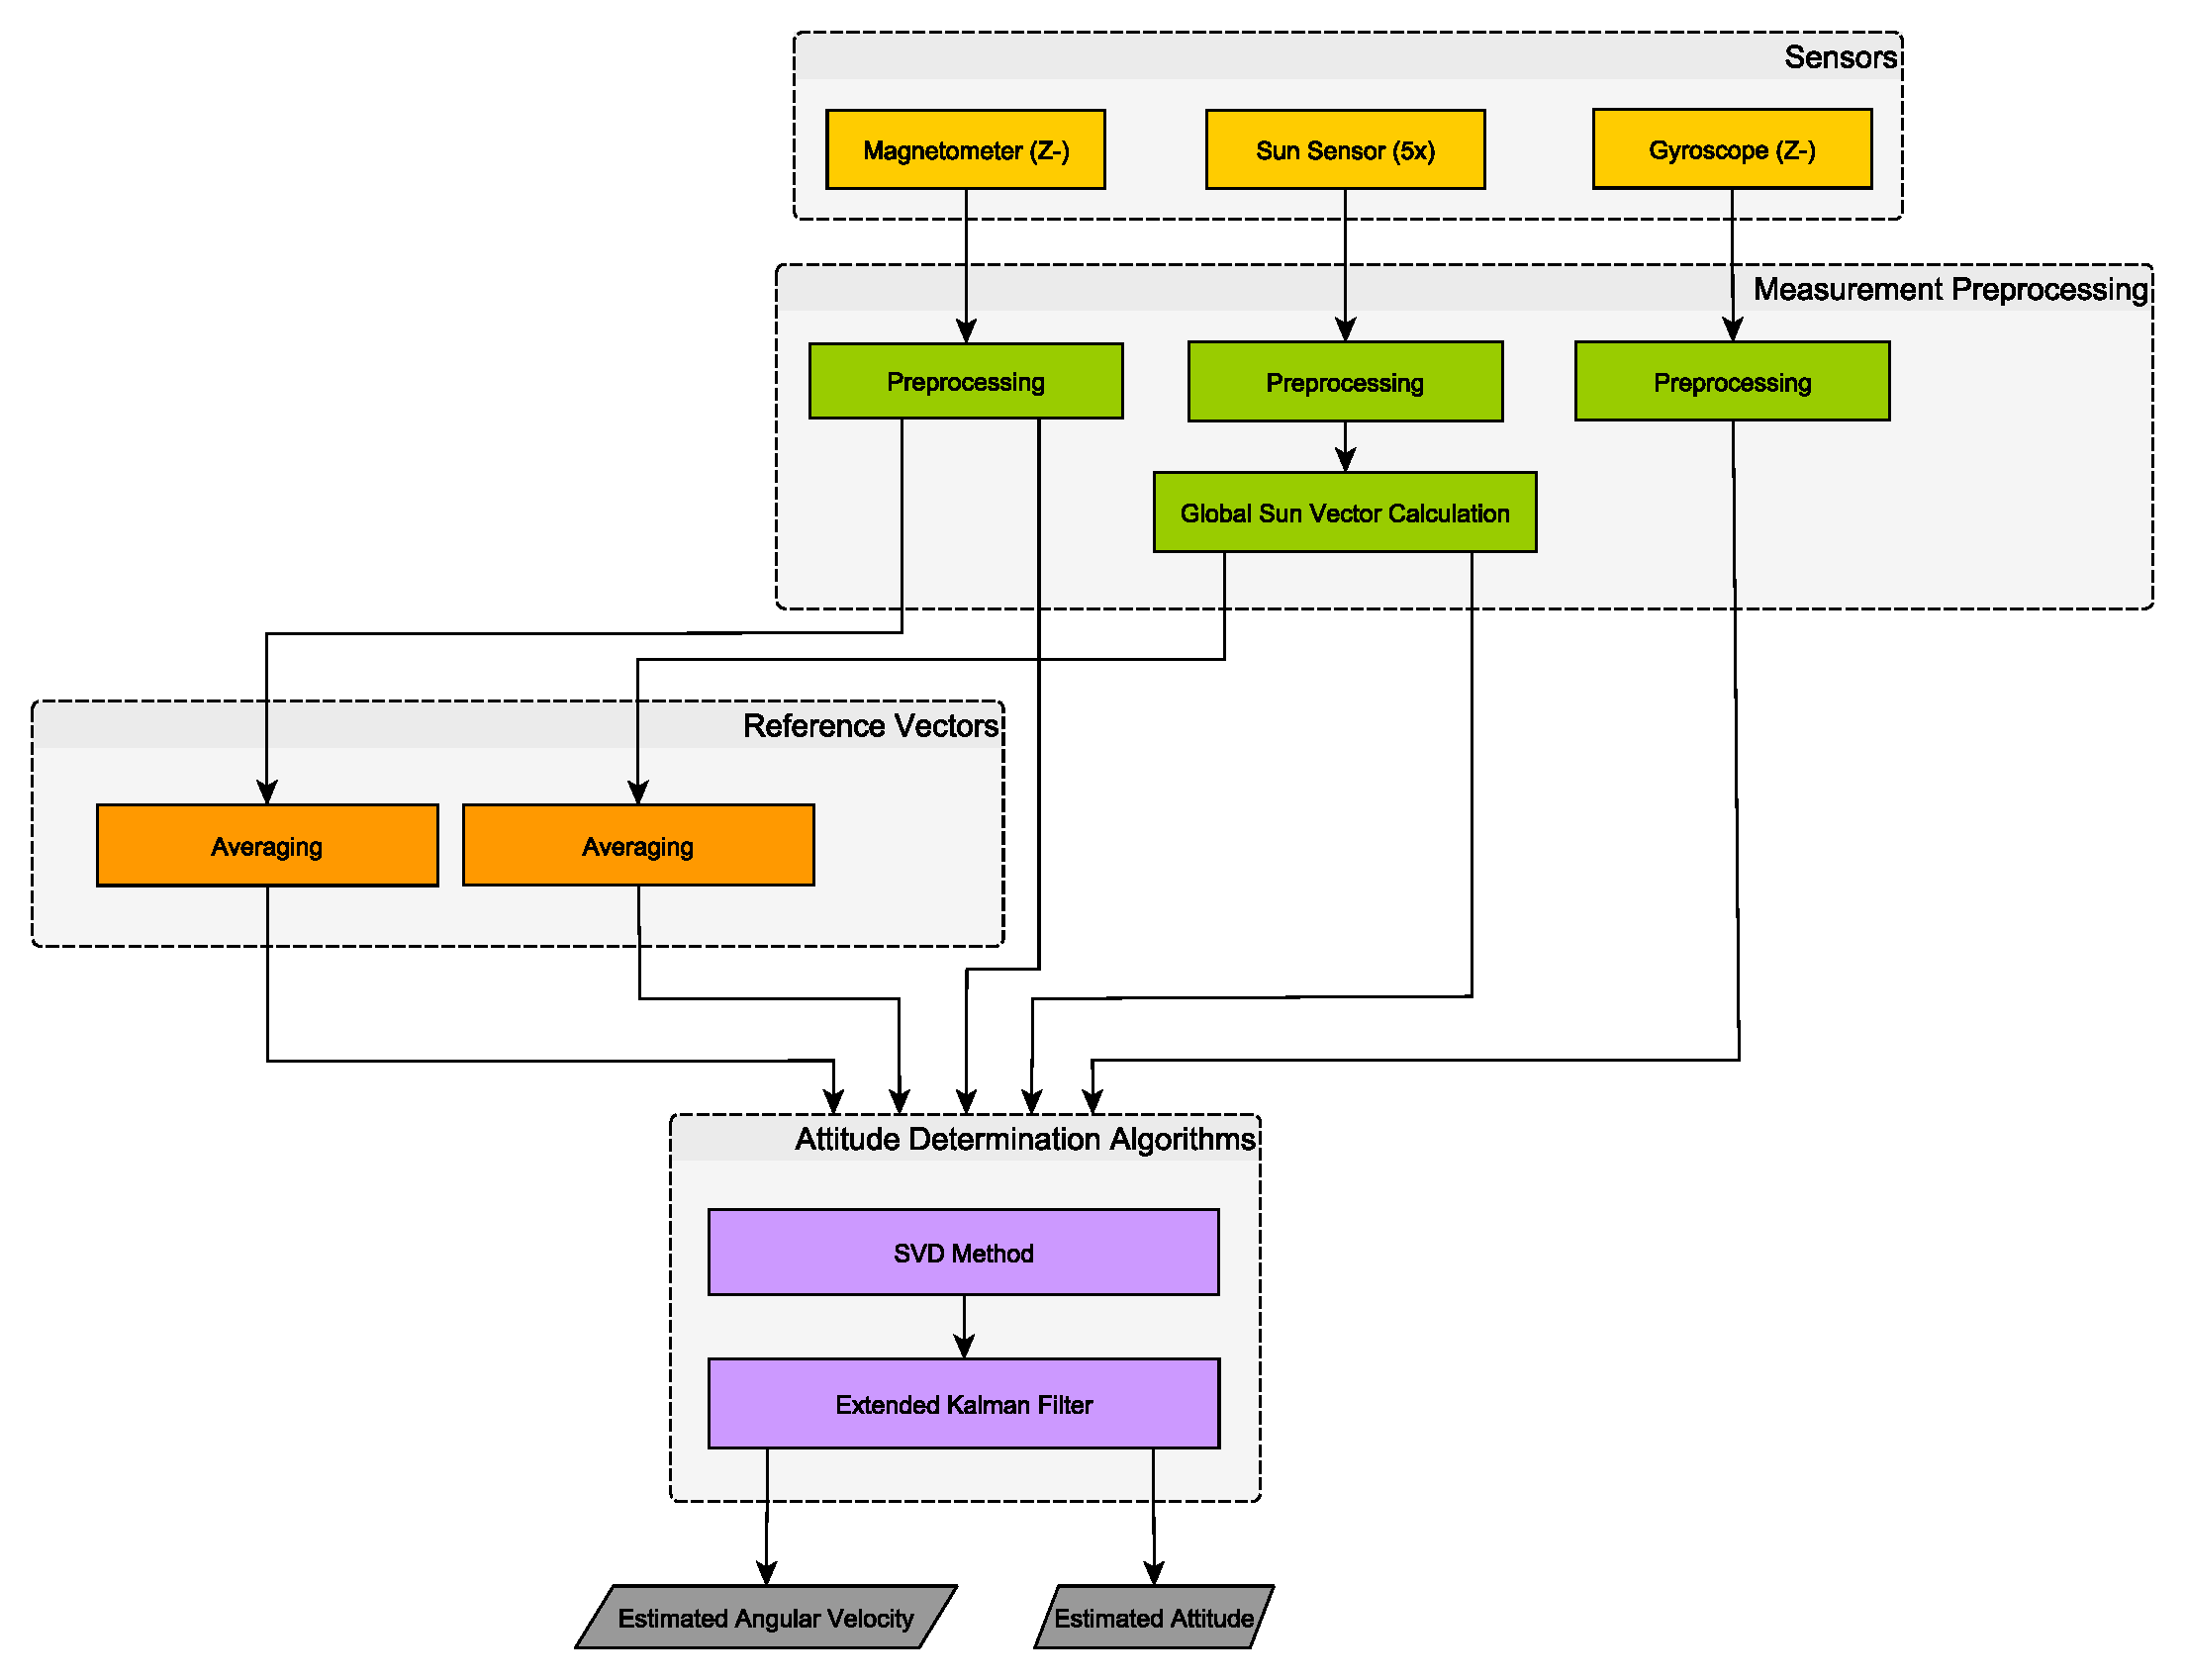
\includegraphics[width=0.7\columnwidth]{./Pictures/ATTDET_Architecture_Ao}
	\caption{An overview of the ADS system when conducting the Algorithm Only test from \cite{DavidThesis}.}
	\label{fig:outdoorOverview}
\end{figure} 

\paragraph{Helmholtz-Cage Approach}
The Helmholtz-cage approach uses a Helmholtz-cage to generate a magnetic field similar to the on expected in the orbit of MOVE-II. The satellite can then be positioned in such a way that the top panel will point directly at a light source representing the sun. As shown in \autoref{fig:Helmholtz-Cage}. By having the top panel face directly at the sun it will be similar to the situation of the satellite having achieved perfect sun pointing. As such all the reference models can be used. This approach has the advantage that none of the firmware has to be changed. The problem is achieving this setup. There is a great uncertainty surrounding the precision of the Helmholtz-cage at the LRT and it is not certain that the cage is able to produce the required magnetic field with an acceptable error. There is also currently no good way of synchronizing the magnetic field model on the satellite and the one used by the Helmholtz-cage to decide what magnetic field to set up. Without this synchronization the test can not be executed. 

\begin{figure}[tbp]
	\centering
	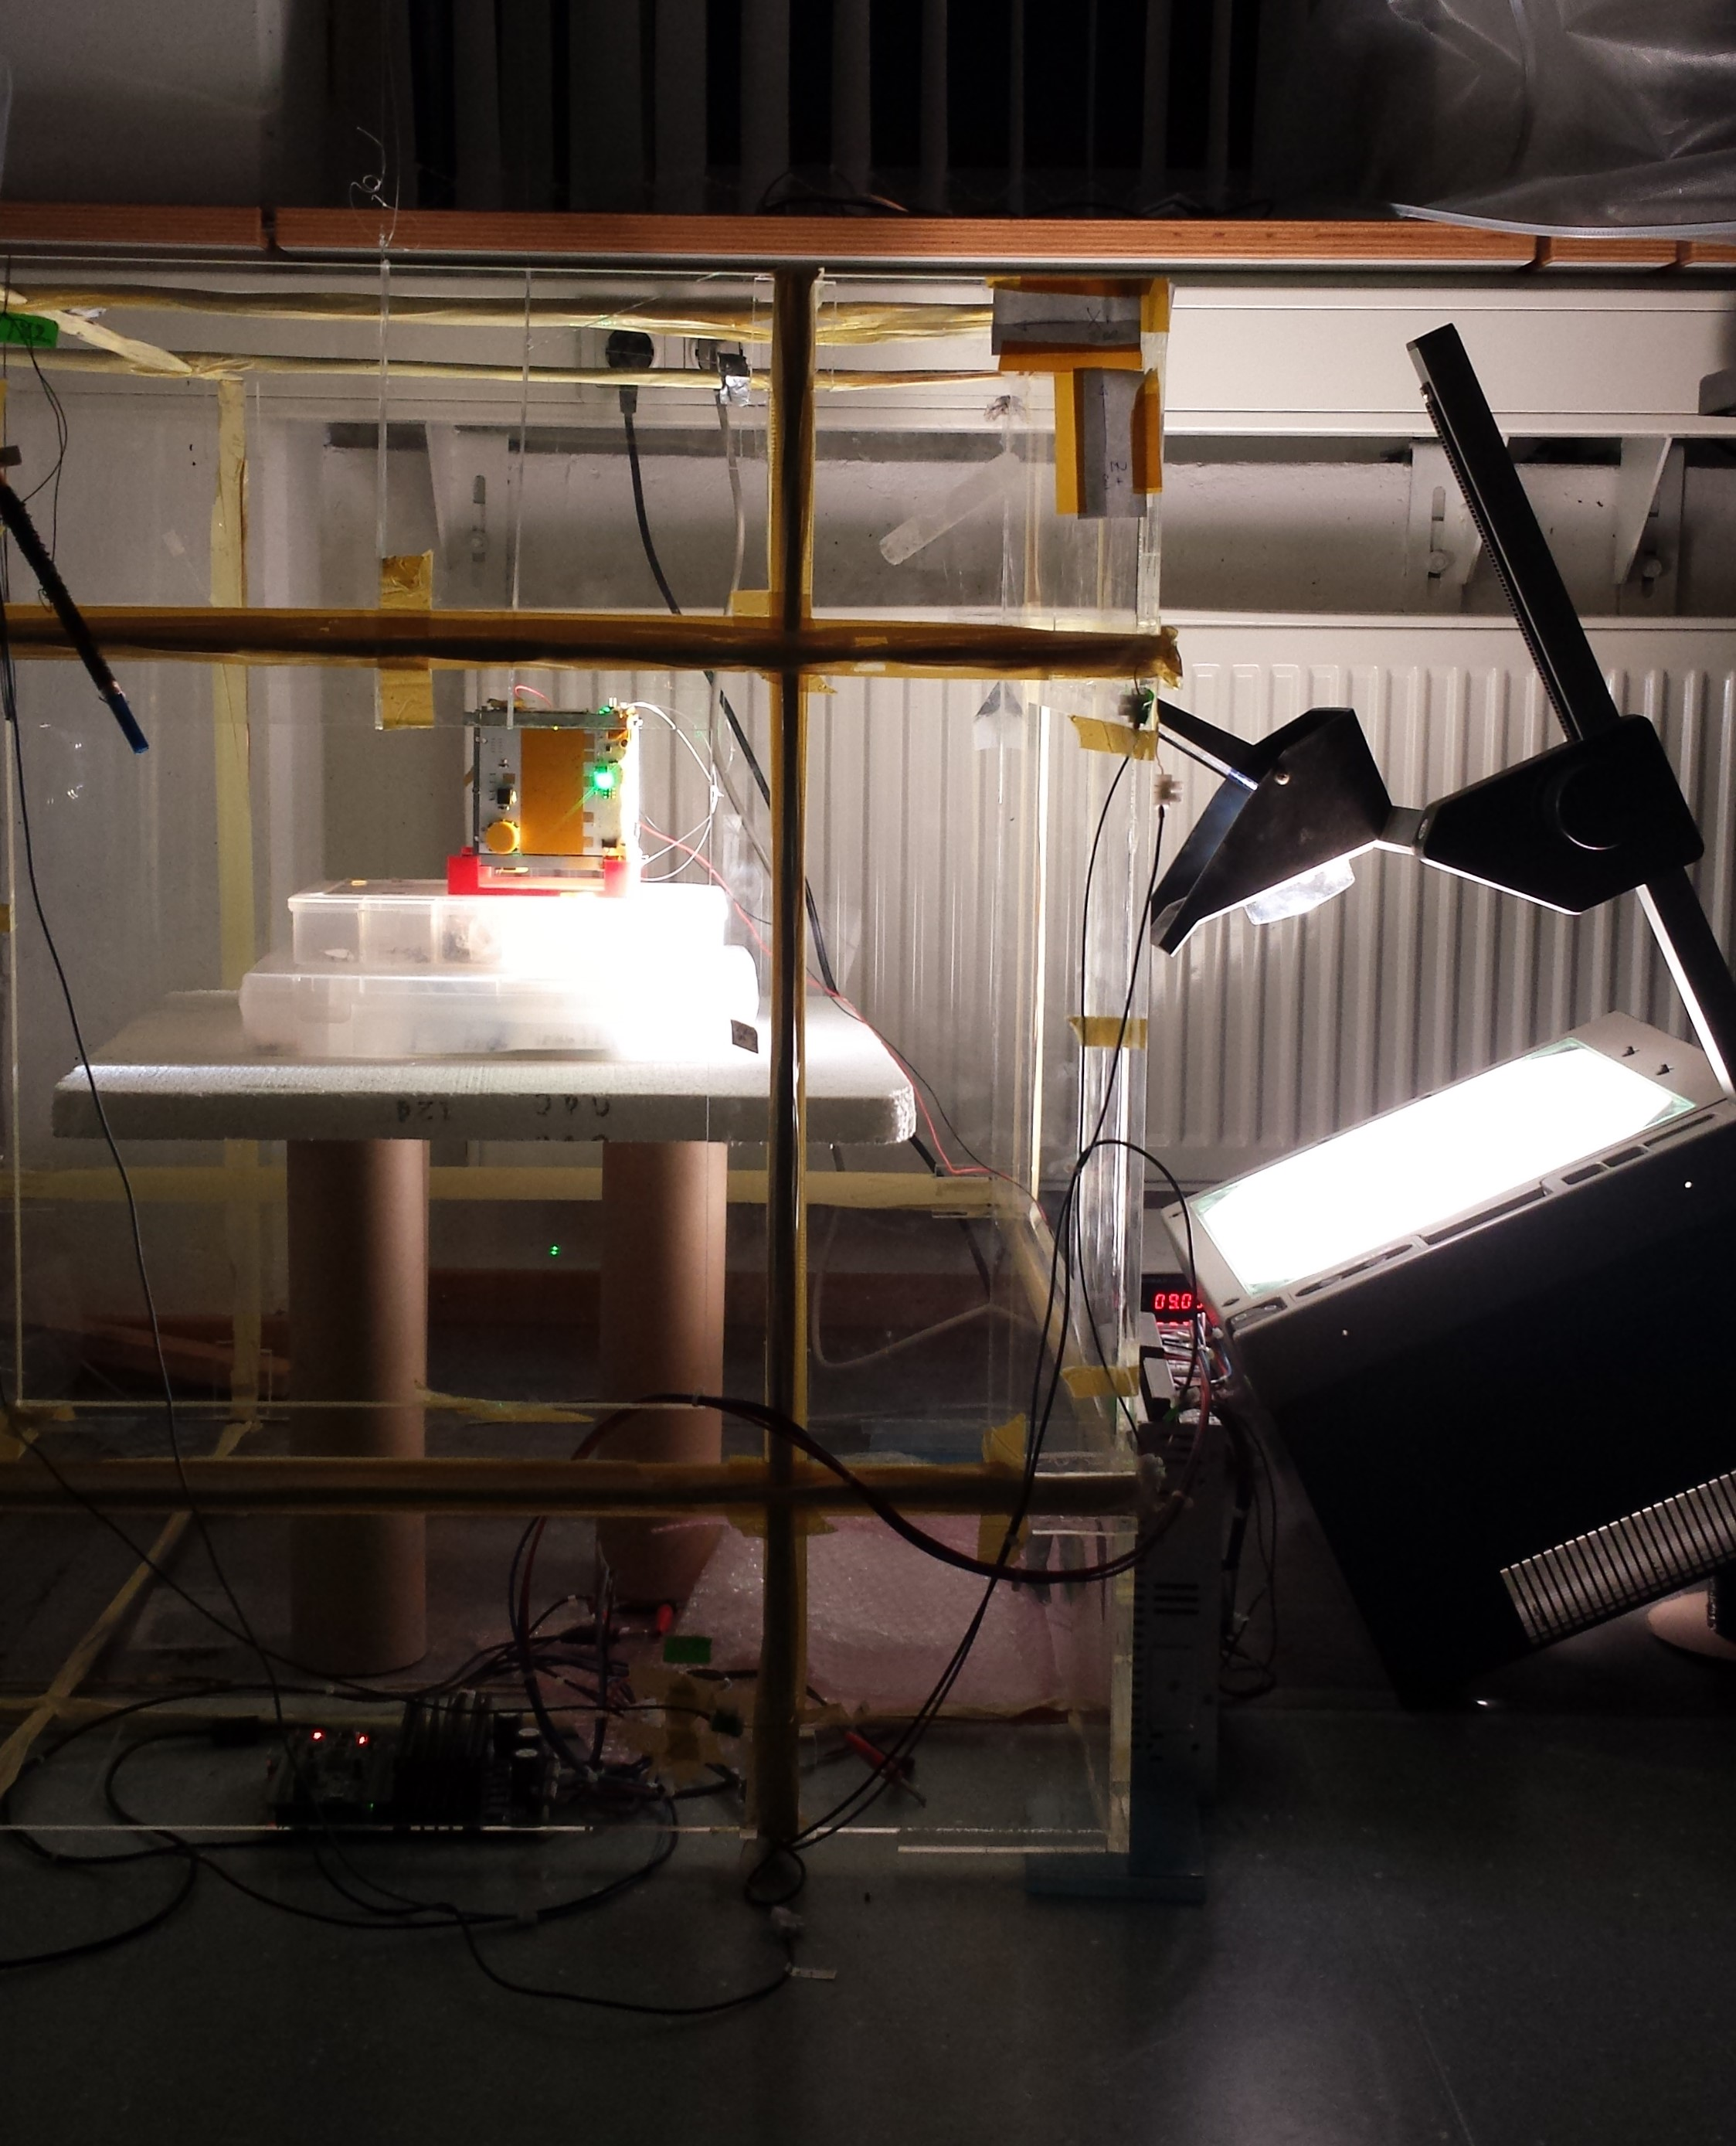
\includegraphics[width=0.3\columnwidth]{./Pictures/Helmholtz_night}
	\caption{Satellite positioned in Helmholtz-cage for ADS testing \cite{DavidThesis}.}
	\label{fig:Helmholtz-Cage}
\end{figure}               

\paragraph{Outdoor}
The outdoor test is simply to take the satellite out on a sunny day. Using the earths magnetic filed and the sun as inputs to the sensors. As both the magnetic field model and sun position model also works for positions on earth the models can be used. Some care has to be taken in choosing a spot with little magnetic disturbance. Some firmware changes are necessary for this test. First of all the satellite is not moving relative to the ECEF frame any more. So the orbit propagator needs to be disabled and a constant position has to be give to the IGRF. Leading to an overview of the ADS as shown in \autoref{fig:outdoorOverview}. The position of the satellite also has be expressed in the ECEF frame. This test has the advantage that it uses almost the entire ADS system. Especially important it that it test all reference models acting with real sensor data. A big disadvantage of this test is that it requires substantial effort to set up as all the equipment has to be brought outside. Also it is reliant on good weather. All this factors makes it unsubtle for intensive debugging, but a good test to test large parts of the system working together.         

\begin{figure}[tbp]
	\centering
	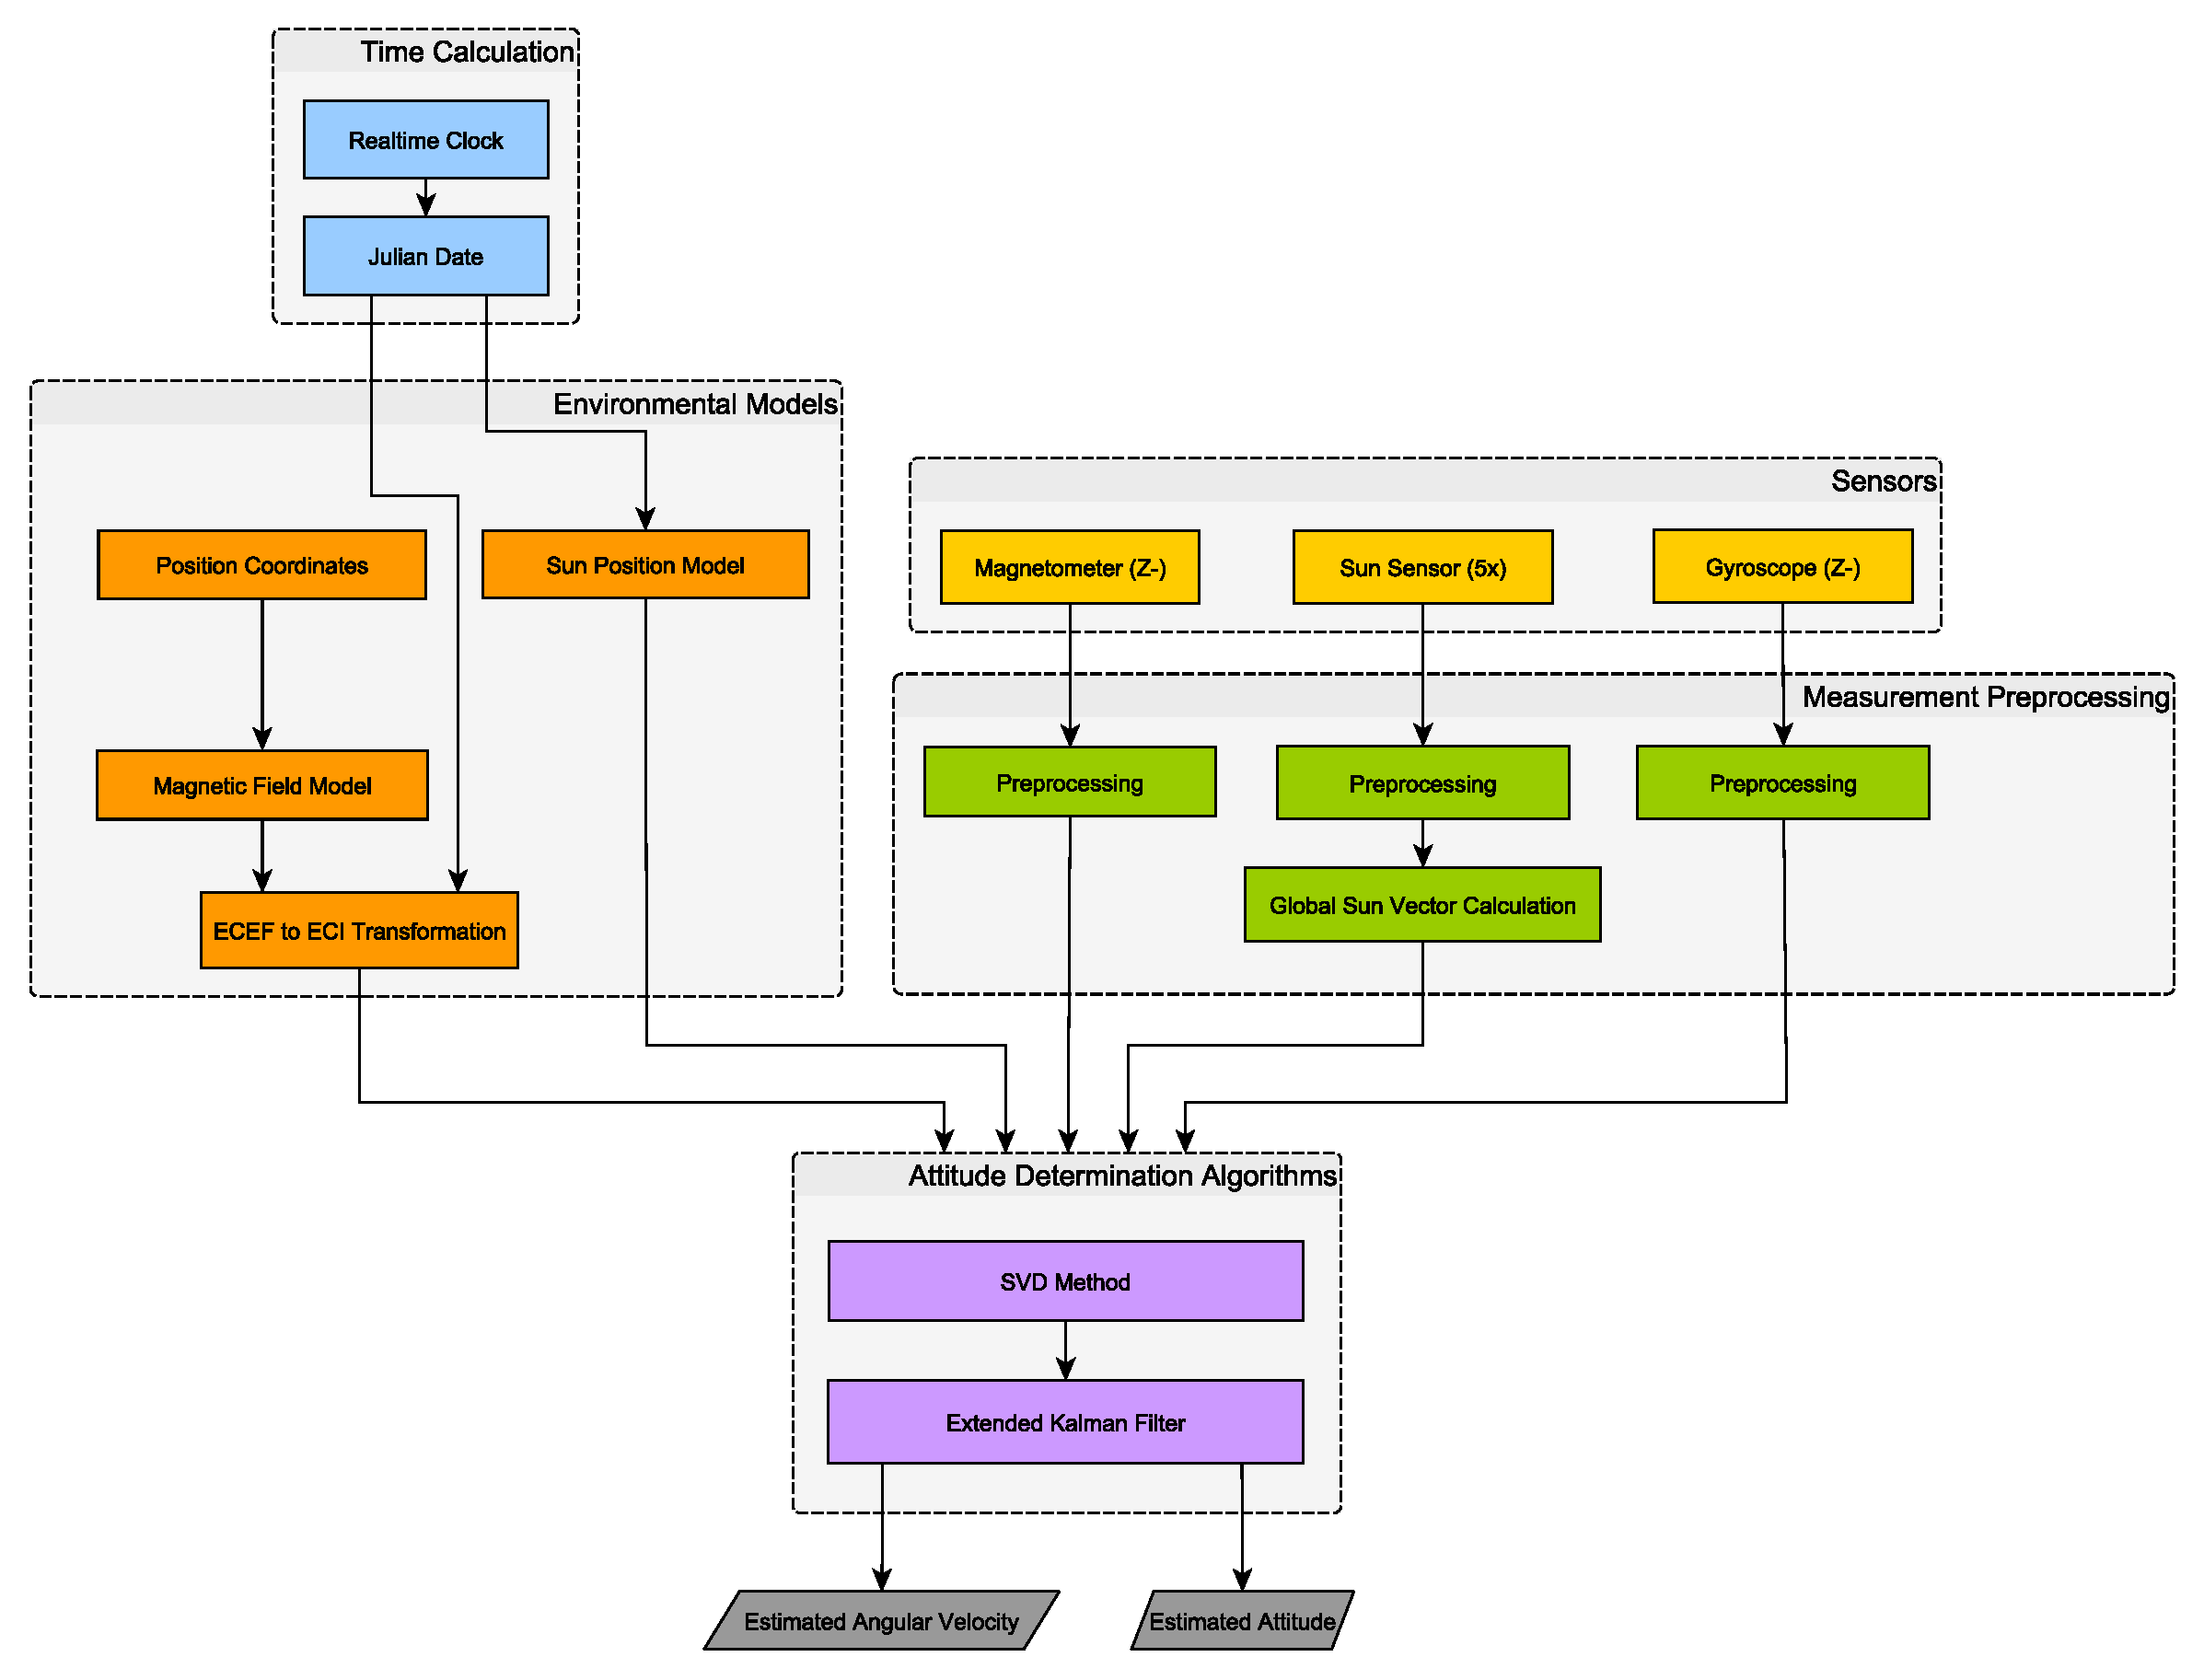
\includegraphics[width=0.5\columnwidth]{./Pictures/ATTDET_Architecture_O}
	\caption{Overview of the ADS when conducting the Outdoor test from \cite{DavidThesis}.}
	\label{fig:outrdoorOverview}
\end{figure}

\paragraph{UWE-3 Laboratory Approach}
The UEE-3 laboratory approach is described in \cite{UWE-3}. The test requires a turntable, Earth's magnetic field and a suitable light source representing the sun. The main idea is to place the light source a suitable place in the laboratory and then adjust the time on the satellite so the position of the light source will be consistent with the reference models of the sun position. This works because the position of the sun is only depends on time so any reasonable position of the light source should also be a position of the sun in the sun position model given the right time. To find this time a matching algorithm was developed by the UWE-3 team it calculates the time based on the three measurements light source elevation angel, angel between magnetic field and light source and the azimuth of the light source. This approach was not chosen because there was no access to a suitable light source and the time investment to develop the algorithm to find the right time was considered to large.

\subsection{Implementation}
The tests where first and primarily implemented on what is called the PrintSat before they were tested on the Flight Model (FM). The PrintSat is described in more detail later in this section. The PrintSat was primarily used because it is a lot easier work with and is more readily available to the ADCS team as it belongs to the team. It is also more suitable for experimenting as it is not as critical if the PrintSat breaks.     

\paragraph{PrintSat}
The PrintSat is a test satellite developed by the ADCS team of MOVE-II. It only contains the elements of the satellite relevant for the ADCS and have been used extensively for testing various parts of the ADCS. The PrintSat contains all the panels that make up that ADCS system, namely the four side panels, the top panel and the main panel. So functionally it has all the same functionality as the ADCS on the FM. The panels are hold together in a cube like construction shown in \autoref{fig:printsat}. In addition the to the ADCS element the PrintSat also contains a beaglebone that is used to represent the main computer on the satellite and the power supply. The beaglebone and the ADCS communicate over SPI in the same way that the ADCS communicates with the rest of the satellite on the FM. This means the ADCS on the PrintSat can be controlled with commands in the same way as on the FM. There also exists an UART connection between the beaglebone and the ADCS that allows additional data to be recorded when using the PrintSat. The power supply also contains a battery so the PrintSat can function with out an external power source. In addition the beaglebone contains a WiFi unit meaning the PrintSat can be connected to a wireless network and reached over an SSH connection allowing for wireless control of the PrintSat. 

\begin{figure}[tbp]
	\centering
	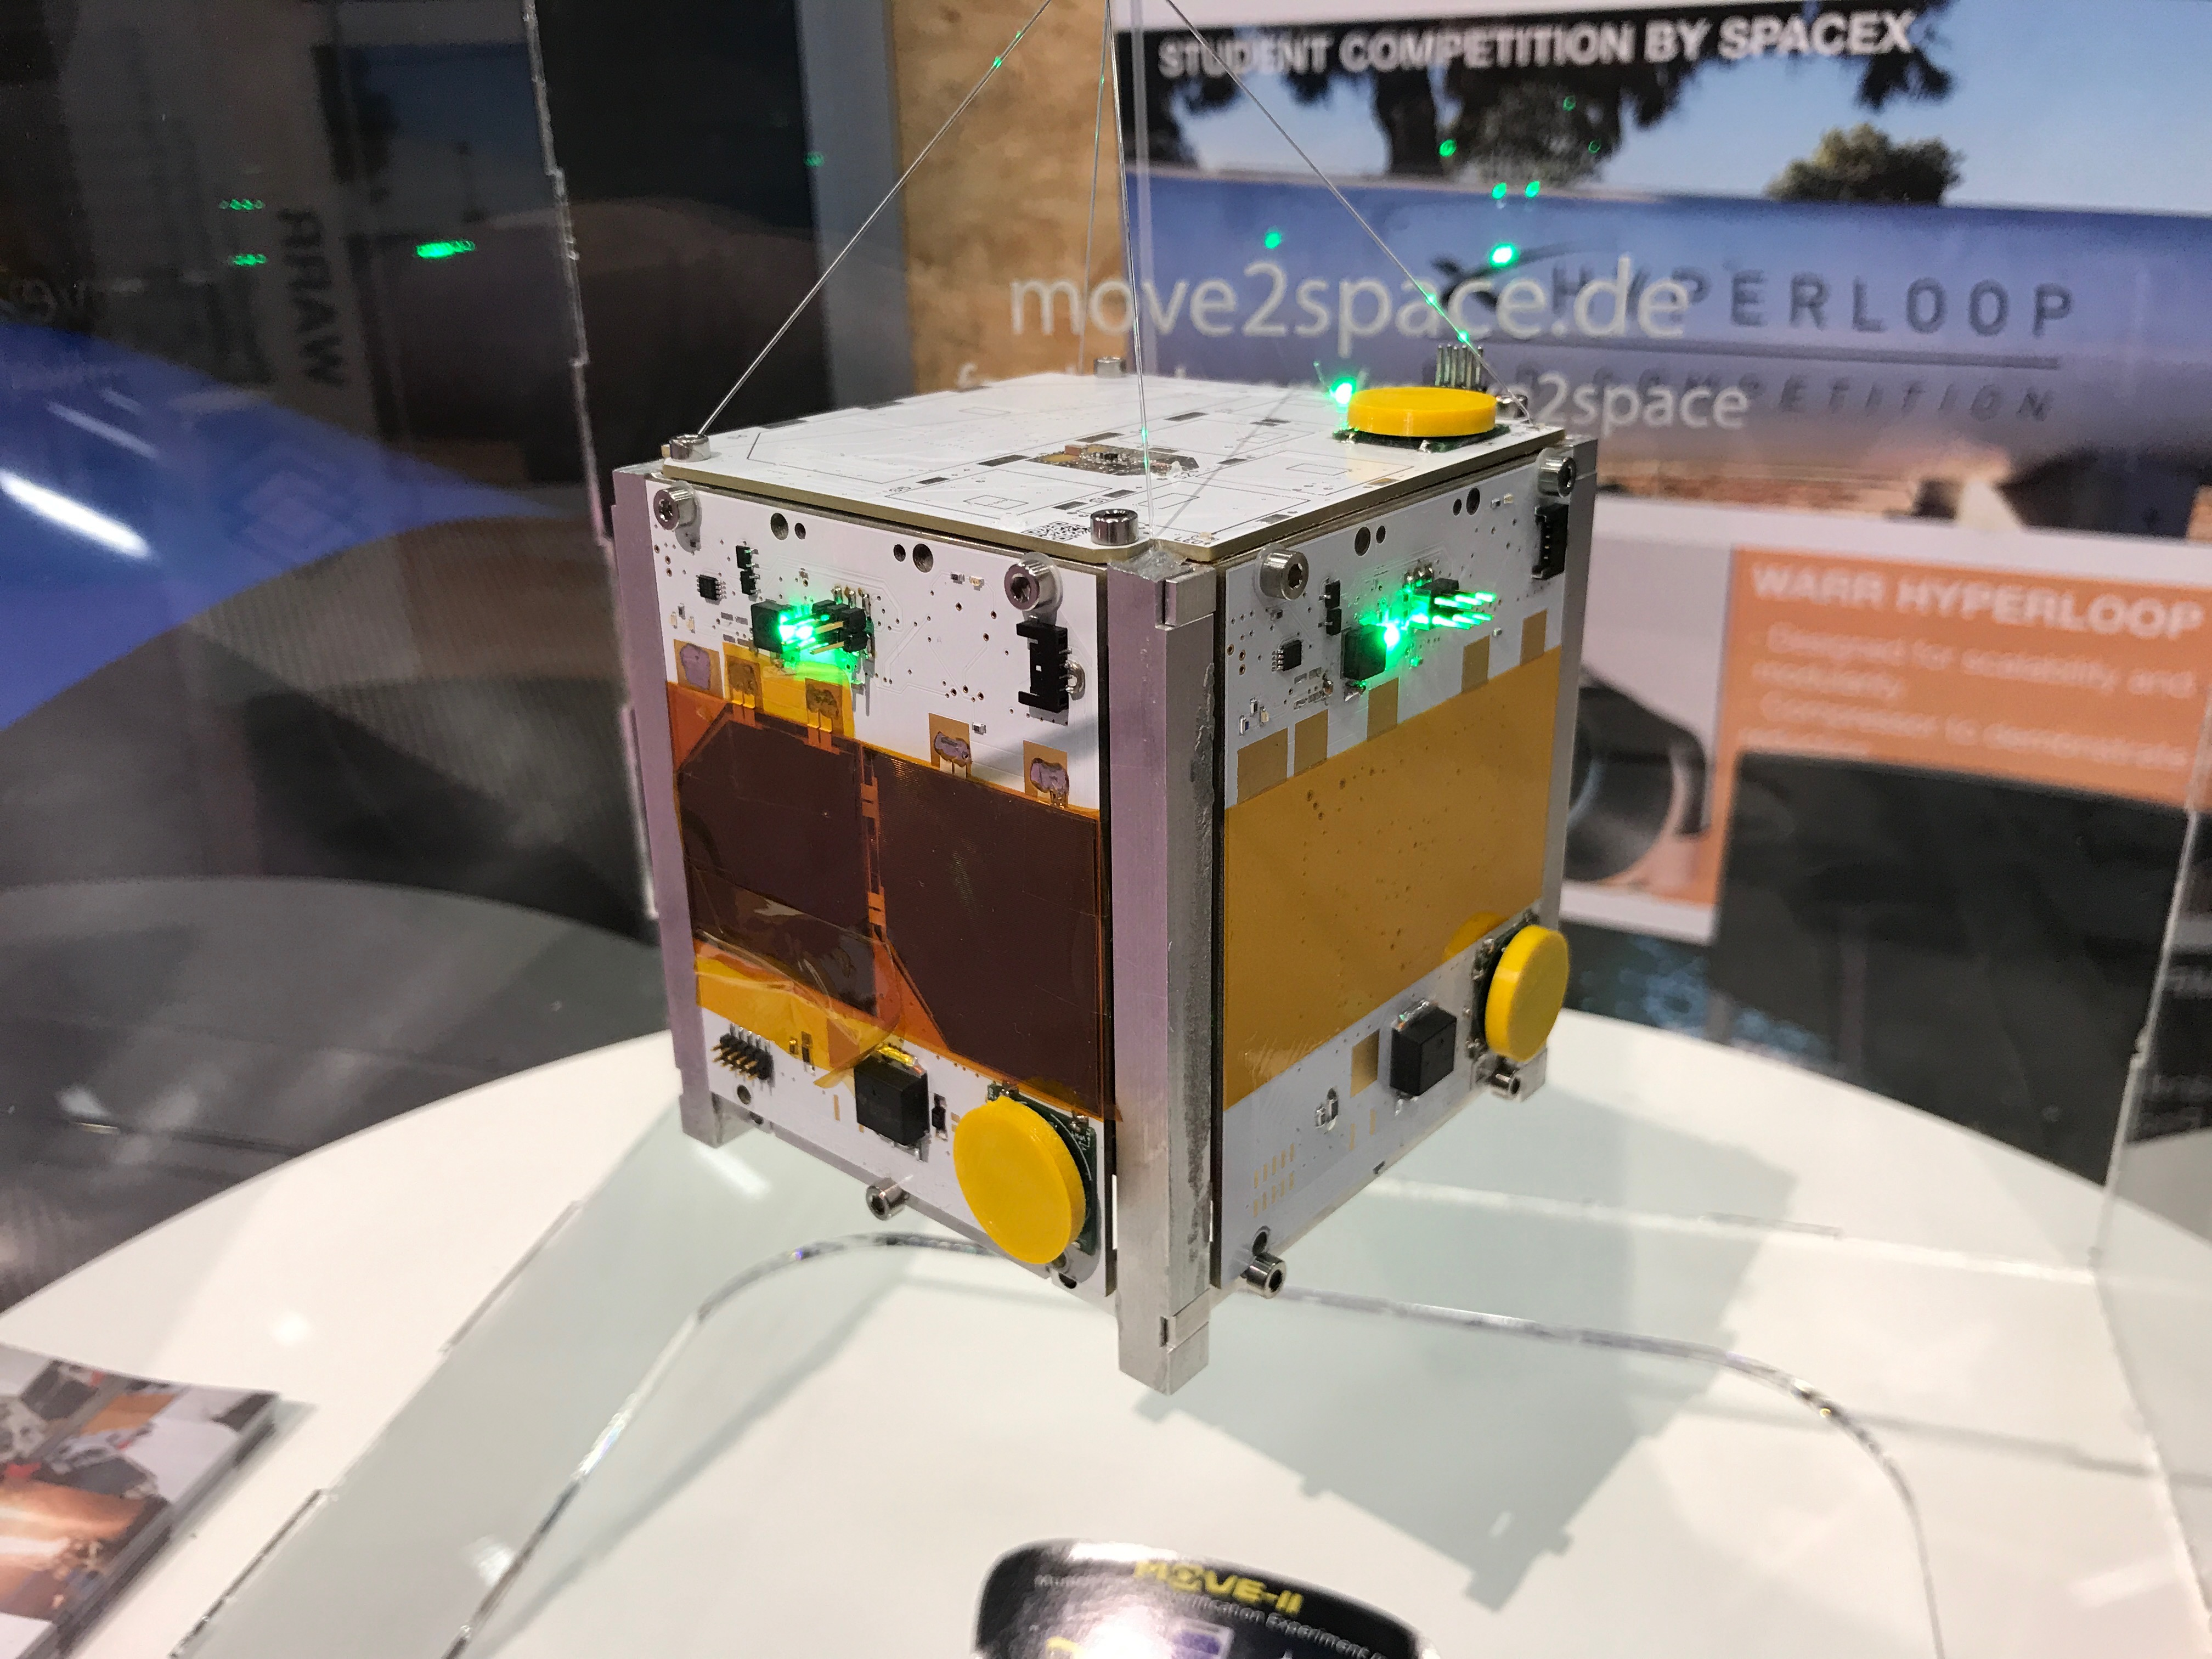
\includegraphics[width=0.5\columnwidth]{./Pictures/printsat2}
	\caption{PrintSat from \cite{DavidThesis}.}
	\label{fig:printsat}
\end{figure}

\subsubsection{Implementation of Algorithm Only}
To implement the Algorithm Only approach some small changes to the ADCS firmware was necessary to disable the reference models and replace them with the averaging function to create the lab frame as described in \autoref{chap:HardwareOnly}. The firmware was also extended with additional debug outputs over a UART connection as the data in the housekeeping files are not sufficient for debugging and proper characterization of the ADS. It should be noted that the data gathered over UART is only accessible on the PrintSat as the FM does not have a UART connection.

The Algorithm Only approach was implemented in a laboratory. A turntable was used to give the satellite a known rotation. The approach also requires a light source. For the light source an overhead projector was used. The overhead projector has been used in previous test of the ADCS. A picture of the test setup can be seen in \autoref{fig:AlgorithmOnlyTestSetup}. With the turntable and the overhead projector different variations can of the test can be set up. Where the variations include static or rotating test with our with out light. Where with light represents when the satellite is in sun and no light represents when the satellite is in the shadow side of the Earth. 

\begin{figure}[tbp]
	\centering
	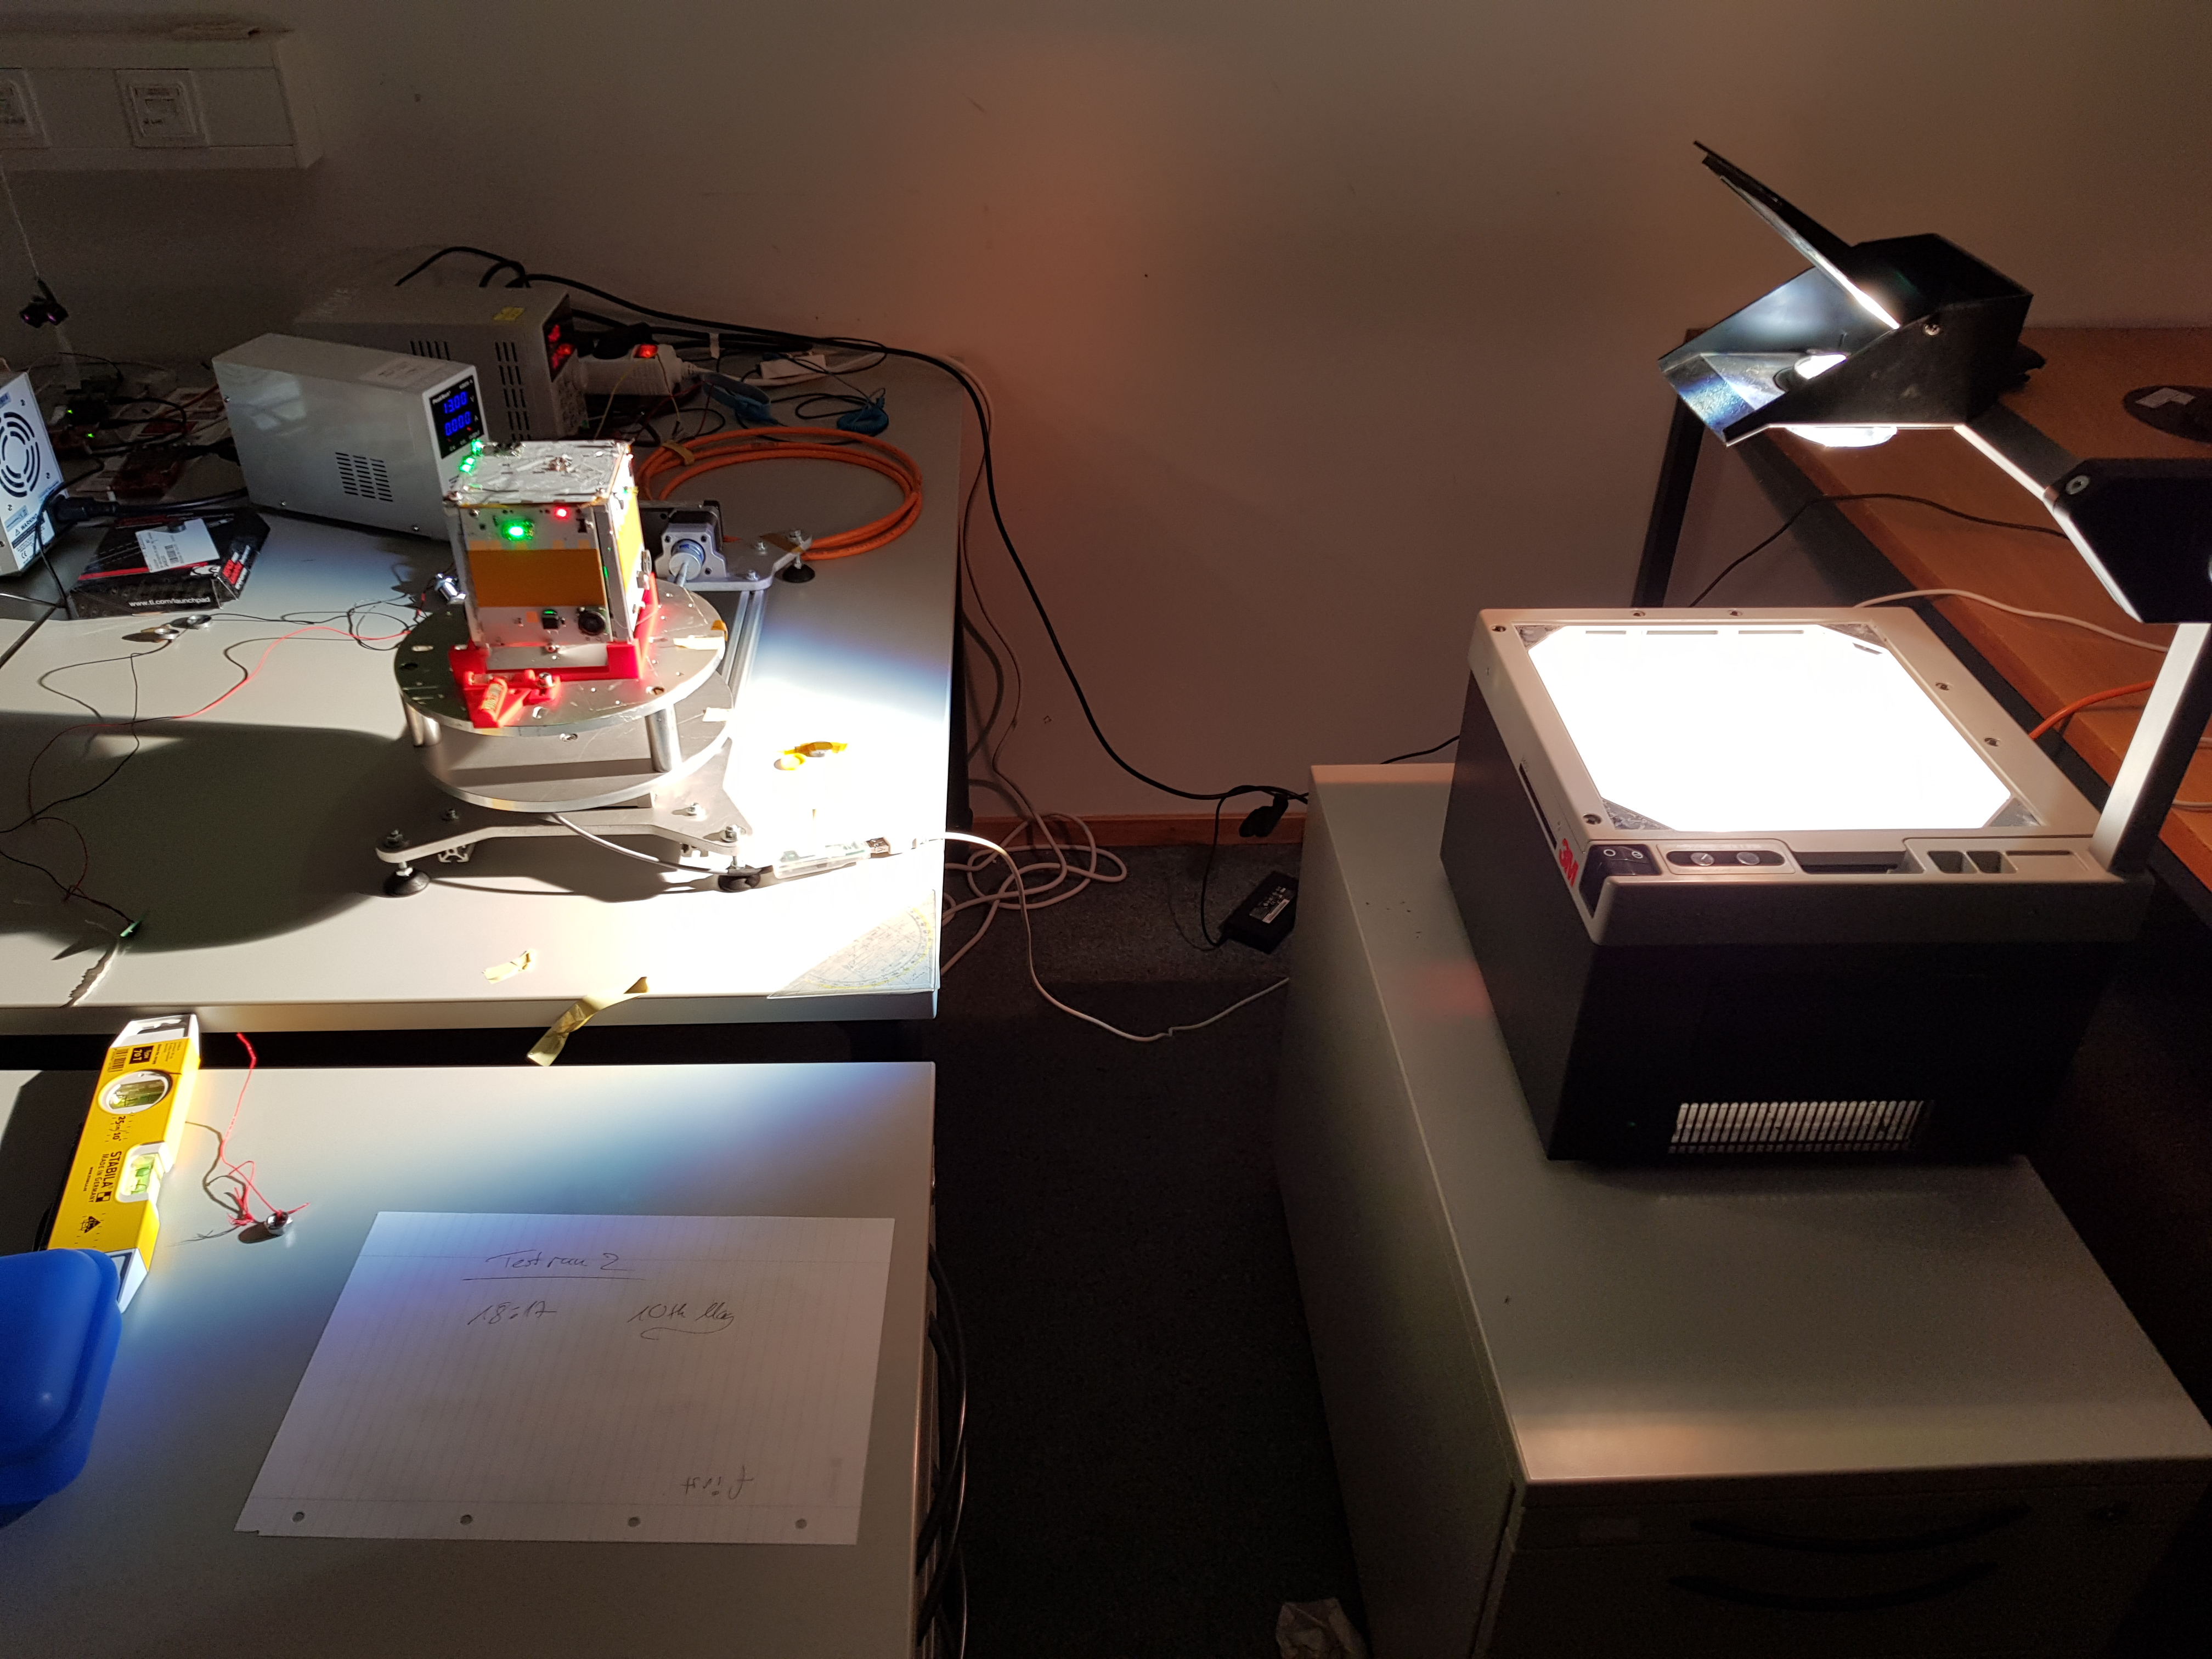
\includegraphics[width=0.5\columnwidth]{./Pictures/Indoor}
	\caption{Algorithm Only setup with the PrintSat from \cite{DavidThesis}.}
	\label{fig:AlgorithmOnlyTestSetup}
\end{figure} 

Before the tests where started the turntable where leveled using a water level. Once the satellite was leveled the recording service both for housekeeping data and the data transmitted from the ADCS to the beaglebone over UART is started. The satellite was then put in attitude determination (ATTDET) mode. The satellite is stationary for some time to generate the new reference frame, after that the turntable can start to turn if it is a rotating test. It is also a possibility to reinitialize the the EKF parameters during the test. After the test the recorded data can be transfered from the PrintSat to a PC for post processing. The time when the turntable is started and stopped is also recorded so it is possible to recreate the rotation of the turntable to have a reference to compare the estimated quaternion with. 

\subsubsection{Implementation of Outdoor}
For the outdoor approach some changes to the firmware had to be implemented. The propagator had to be disabled and a constant position had be be given to the IGRF model. It was also necessary to do some more changes to the debug output and the housekeeping data. This is because the output from the ADS when all models are used is the quaternion representing the rotation between ECI and body-fixed frame. This data is hard to interpret, so a new frame was defined. This frame called the lab frame is defined as North East Down (NED) so the x-axis points north, the y-axis points east and the z-axis completes the right hand rule by pointing down towards the earth. This frame is much easier to analyze as it is easy to align the fixed-body frame with the lab frame. To get the quaternions to represent the rotation between the lab frame and the fixed-body frame a simple transformation is needed. In the ADS there already exist a function to go from ECI to ECEF frame. The transformation between ECEF and the lab frame can be accomplished by the rotation matrix shown in \autoref{eq:ECEFtoLab} according to \cite{UWE-3}. Where $\Phi$ is latitude and $\lambda$ is longitude of the position where the test is conducted. The decision to do this calculations live on the satellite instead of in post processing was mainly due to the fact that the ECI to ECEF transformation is time dependent and it would be difficult to get the synchronization correct.    

\begin{equation}\label{eq:ECEFtoLab}
	\boldsymbol{R}_{LE} = \begin{bmatrix}
		-sin(\Phi)cos(\lambda) & -sin(\Phi)sin(\lambda) & cos(\Phi) \\
		-sin(\lambda) & cos(\lambda) & 0 \\
		-cos(\Phi)cos(\lambda) & -cos(\Phi)sin(\lambda) & -sin(\Phi) \\
	\end{bmatrix}
\end{equation}                       

In the execution of the actual test the satellite and turntable was brought out to a nearby field away from buildings. A WiFi router that could be powered with a micro-usb cable from a computer was also brought. This was to create a local WiFi network so commands could be send to the PrintSat. The body frame of the satellite was then aligned as good as possible to the lab frame. This was done by using a water level to level the satellite and by using a simple compass to align the x-axis of the satellite as good as possible to the north. A picture of the setup can be seen in \autoref{fig:OutdoorTest}. Once the satellite was aligned with the lab frame the data recording services where started before the satellite was put into ATTDET mode. The EKF can also be reinitialized by a simple command. Then the turntable could start turning if it was a rotating test. It should be noted that there are no successful rotation outdoor tests as there was some difficulty getting the turntable to work with the mobile power source. Tests of when the satellite is in the shadow of the Earth can also be conducted by increasing the threshold of the sun sensors to a very high value. This means that none of the recorded sun sensor data will be accepted as valid and will therefore not be used in the EKF. This is similar to what will happen once the satellite is on the shadow side of Earth. It should be noted that for this test setup it is very important that the sensors are properly calibrated and that the time on the satellite is correct. In contrast to the Algorithm only test where calibration and satellite time does not matter.

\begin{figure}[tbp]
	\centering
	\includegraphics[width=0.5\columnwidth]{./Pictures/Outdoor}
	\caption{Outdoor test setup with the PrintSat from \cite{DavidThesis}.}
	\label{fig:OutdoorTest}
\end{figure}

\ifdraft
\section{Test Results}
Only the test result from the Hardware-only test will be presented, to get an overview of the different simulation test see \cite{DavidThesis}. The analysis of the result will also be more qualitative than quantitative. For a more quantitative approach see \cite{DavidThesis}. For the PrintSat there will be result for both the Algorithm only and Outdoor test, for the FM there are only results from the Algorithm only test as it was not possible to conduct an successful Outdoor test before the FM had to be delivered to the launch provider for integration. 

\subsection{PrintSat}
Using the PrintSat with the Algorithm only and Outdoor approach a large portion of the functionality of the ADS has been verified and the confidence in the ADS has increased a lot. The test has also shown some malfunction in the ADS that are currently still under investigation. 

\subsubsection{PrintSat Algorithm Only Results}
The most typical working conditions that the satellite will face in space is spinning with and with out sun light. For those two scenarios the result also look promising. In \autoref{fig:cdr3RotSun} and \autoref{fig:cdr3RotNoSun} you can see the results from a test where the satellite is rotated around it's z-axis three times. Where \autoref{fig:cdr3RotSun} and \autoref{fig:cdr3RotNoSun} is with and with out sun respectively. The dotted lines in the plot is the reference trajectory. The reference trajectory is calculated by rotating a reference quaternion around the z-axis with angular velocity calculated by dividing the total number of revolution by the time taken to couplet the rotations. As you can see from the results both test work reasonably well. The estimated quaternion are able to follow the reference quaternion to an acceptable degree. 

\begin{figure}[tbp]
	\centering
	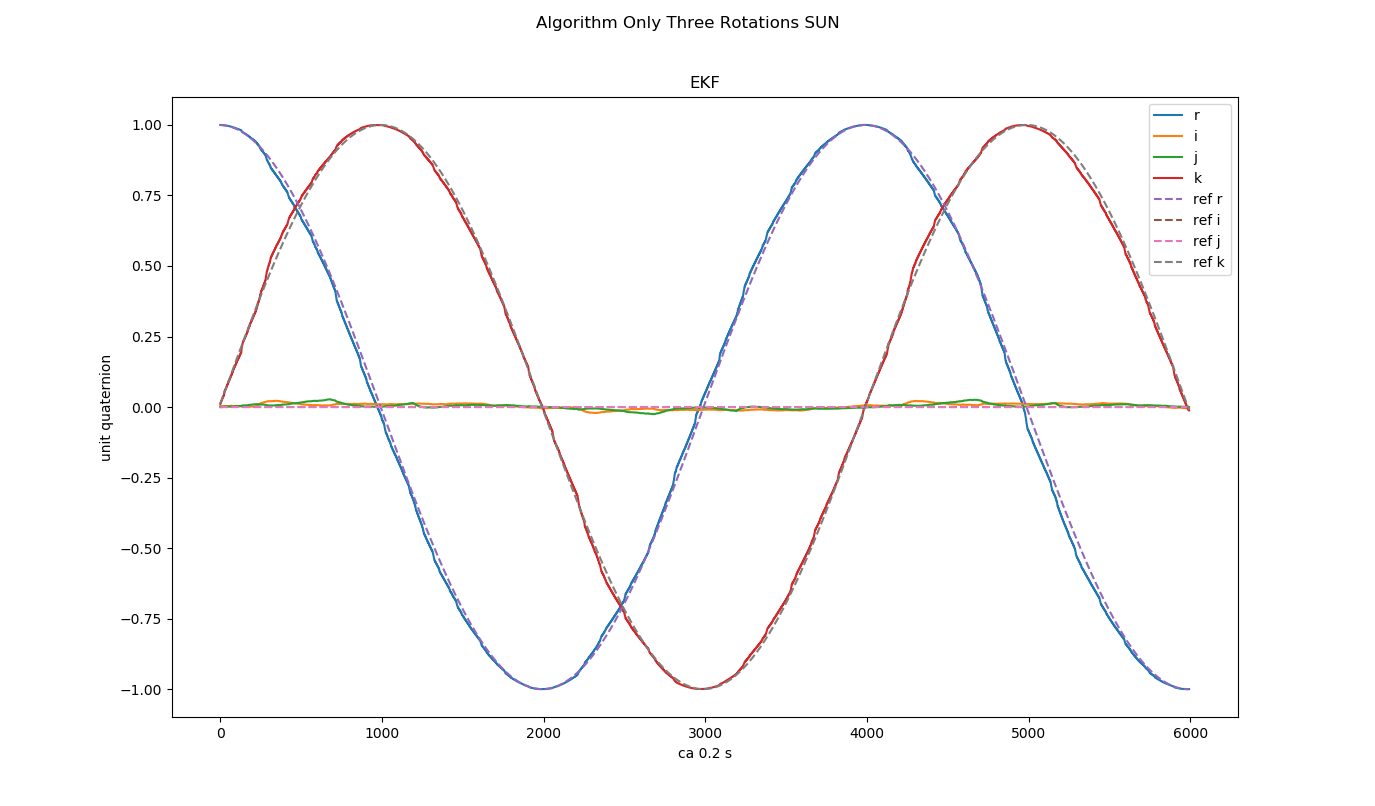
\includegraphics[width=1\columnwidth]{./Pictures/cdrRun3ThreeRotationsSun}
	\caption{Plot of recorded quaternion and reference quaternion for Algorithm only test using the PrintSat. Three rotations with sun}
	\label{fig:cdr3RotSun}
\end{figure}               

\begin{figure}[tbp]
	\centering
	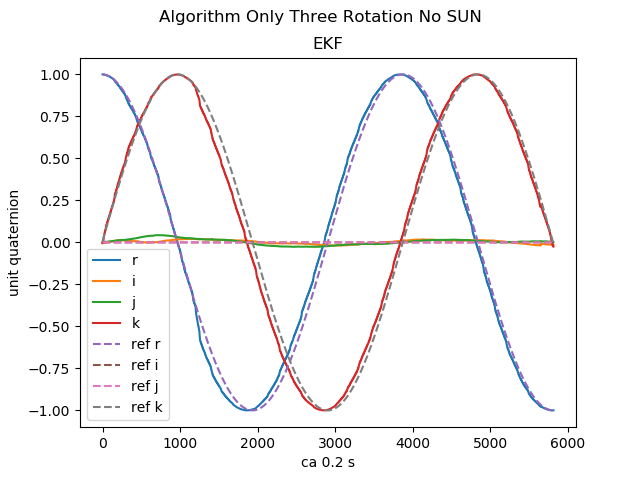
\includegraphics[width=1\columnwidth]{./Pictures/cdrRun3ThreeRotationsNoSun}
	\caption{Plot of recorded quaternion and reference quaternion for Algorithm only test using the PrintSat. Three rotations with  no sun}
	\label{fig:cdr3RotNoSun}
\end{figure}

\subsubsection{PrintSat Outdoor Results}
When conducting the outdoor test there was no possibility of conducting tests with rotations as there was problems getting the turntable to work with batteries. A problem arises when there is no rotation. In \autoref{fig:OutdoorNoRotationSun} which is a test with sun and no rotation it seems to be fine. The recorded quaternion is about $[1 0 0 0]$ which is expected as the PrintSats body-fixed frame is aligned with the lab frame. In \autoref{fig:OutdoorNoRotationNoSun} which is no sun and no rotation the EKF starts to struggle. From the results it seems like quaternions are converging towards the correct values, but the test is too short to say for sure what the quaternions are converging towards. Even if the quaternions are converging towards the right value it is way too slow. For the current implementation of the attitude controller this is not a problem as it is a spinning controller, but one of the main reasons that the EKF is being implemented is to allow for the possibility to implement other types of controllers. One of this future controller could be a non-spinning controller and the EKF should therefore be able to handle this scenario. Even if the problem does not affect the current design and is unlikely to come up in use it is a bug and before the root cause is discovered it is impossible to say what other side effects it might have.

\begin{figure}[tbp]
	\centering
	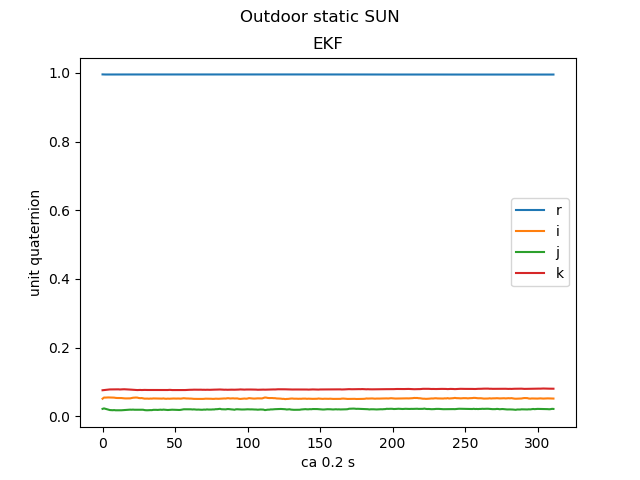
\includegraphics[width=1\columnwidth]{./Pictures/run3OutdoorStaticSUN}
	\caption{Plot of recorded quaternion quaternion for Outdoor test using the PrintSat. Static test with sun}
	\label{fig:Outdoor3RotNoSun}
\end{figure}

\begin{figure}[tbp]
	\centering
	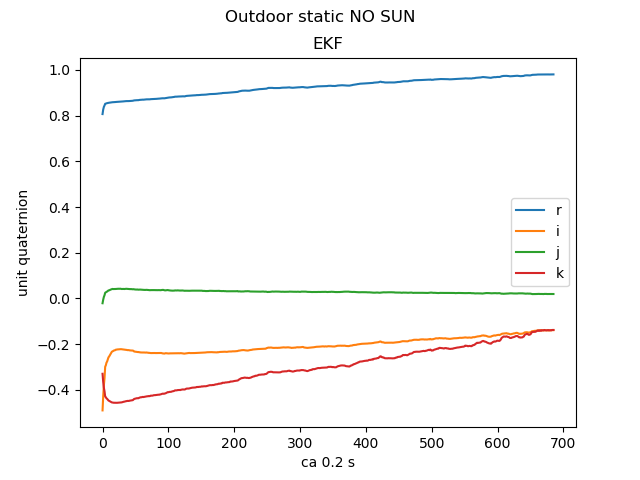
\includegraphics[width=1\columnwidth]{./Pictures/run3OutdoorStaticNOSUN}
	\caption{Plot of recorded quaternion for Outdoor test using the PrintSat. Static with  no sun}
	\label{fig:Outdoor3RotNoSun}
\end{figure}         

Some effort have been put into trying to figure out why this happens. An initial theory is was that it is due to the fact that the EKF is not initialized by the SVD and that it will converge to the right value give enough time. It is just so slow because the initial estimate is so far away from the correct estimate. The problem with this theory is that the ADS seems to work when there is rotation and no sun. In this scenario there is also no SVD initialization, so it seems like the EKF works even with out the SVD initialization. As a part of the future investigation a static Algorithm only test where conducted where the conditions where changed from sun to no sun before it was set back to sun. The results can be seen in \autoref{fig:cdrSunNoSunSun}. The results show that the quaternions stay constant even when there is sun if they have converged to the right values first. This at least indicates that the EKF does not diverge if the quaternions have already converge to the right value. For future investigation the problem have been recreated in simulations. This also indicates that the problem is a problem with the algorithm itself and not the implementation on the satellite or any hardware related issues. 

\begin{figure}[tbp]
	\centering
	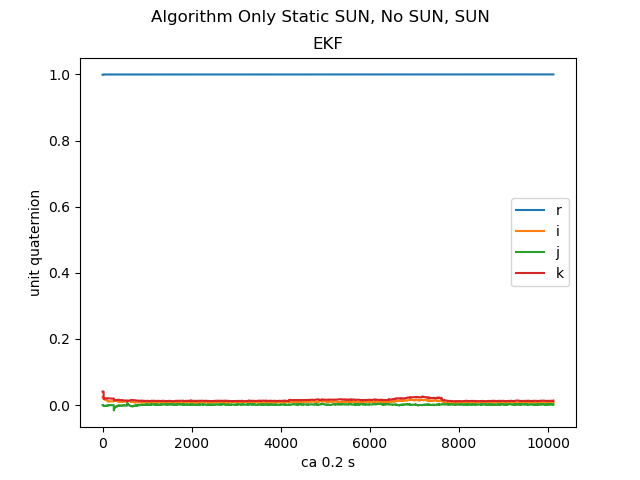
\includegraphics[width=1\columnwidth]{./Pictures/cdrRun1StaticSunEclipsSun}
	\caption{Plot of recorded quaternion for Algorithm only test test using the PrintSat. Static test where the condition are changed from sun to no sun and then back to sun. }
	\label{fig:cdrSunNoSunSun}
\end{figure} 

\subsection{Flight Model}
The test with the FM where limited in scope and mostly to verify that the same behavior that is seen on the PrintSat can be seen on the FM as well. There results from two test shown in \autoref{fig:FMcdrTwoRotSun} and \autoref{fig:FMcdrTwoRotNoSun} show that the results are somewhat consistent with the PrintSat. The overall trend in both is that ADS is preforming reasonably well and the estimated quaternions are able to follow the reference quaternions reasonably well. In \autoref{fig:FMcdrTwoRotSun} the preference is a lot worse than on the PrintSat equivalent test seen in \autoref{fig:cdr3RotSun}. There are this seemingly periodic shifts in the estimated quaternion that was not so viable on the PrintSat. This seems to come from spikes in the sun sensor measurements as you can see in the bottom plot of \autoref{fig:FMcdrTwoRotSun} there is a shift in the estimated quaternion whenever there are spikes in the sun sensor measurement. The spikes in the sun sensor measurements seem to come from when there is a switch in which sun sensor that is being used. The switching comes from a new panel side panel facing the sun. The reason why the spikes in sun sensor measurements are only on the FM and not on the PrintSat is still under investigation, but the working theory is that the spikes comes from the environment. As the FM test was conducted in the integration that is not completely dark while the PrintSat test where done in a complete dark room. 

\begin{figure}[tbp]
	\centering
	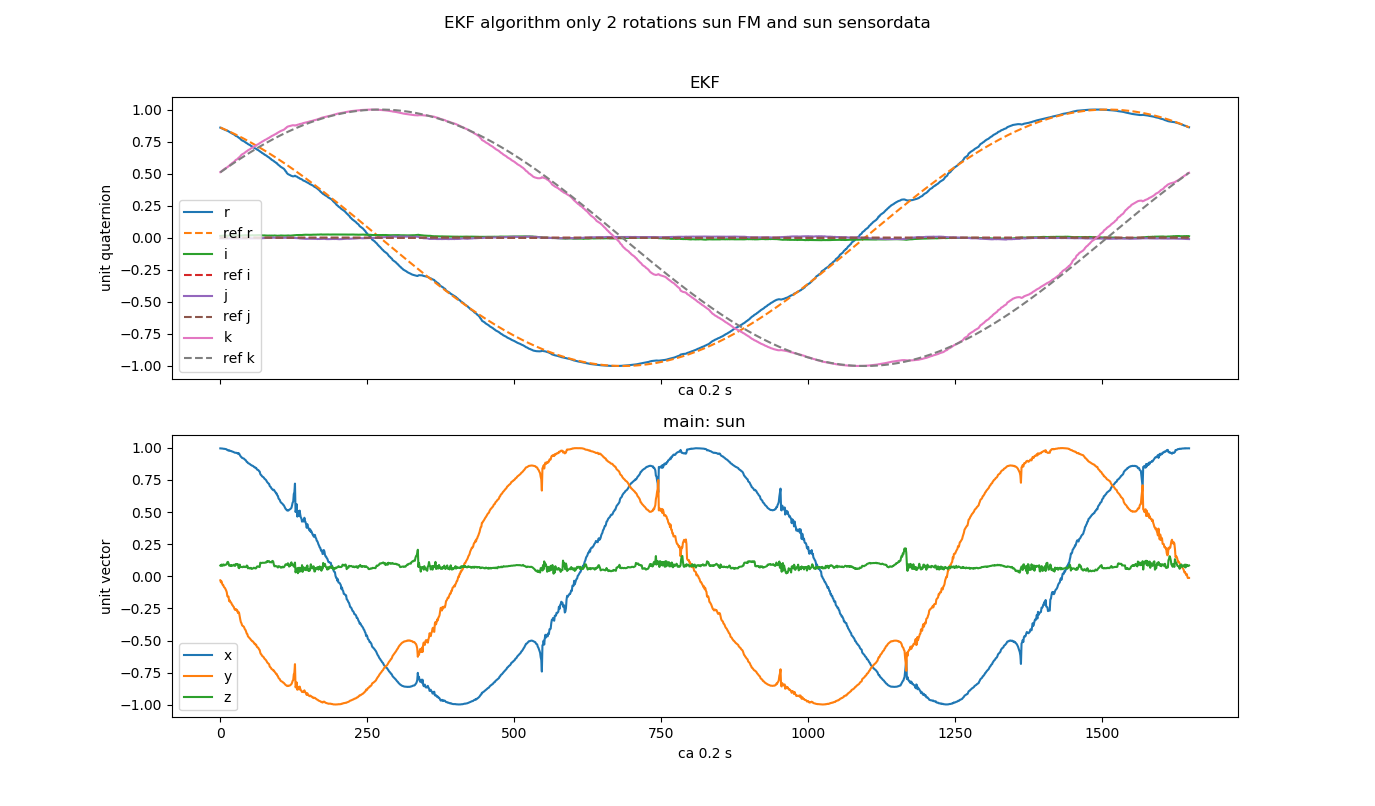
\includegraphics[width=1\columnwidth]{./Pictures/test1EKFandSUN}
	\caption{Plot of recorded quaternion for Algorithm only test test using the FM and the recorded sun sensor measurements. The FM is turned two time on the turntable.}
	\label{fig:FMcdrTwoRotSun}
\end{figure}

\begin{figure}[tbp]
	\centering
	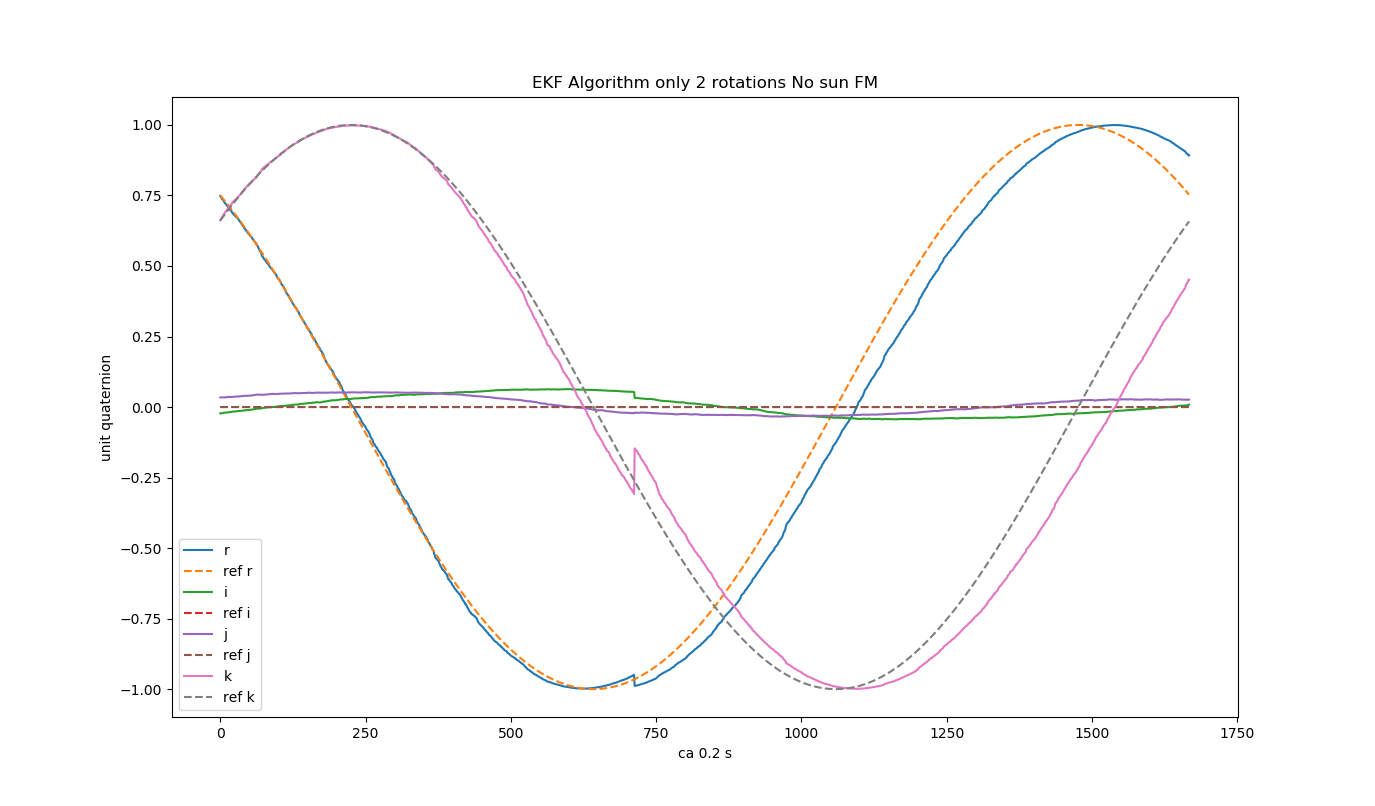
\includegraphics[width=1\columnwidth]{./Pictures/EKF_Algorithm_only_2_rotations_No_sun_FM}
	\caption{Plot of recorded quaternion for Algorithm only test using the FM. The FM is turned two times on the turntable.}
	\label{fig:FMcdrTwoRotNoSun}
\end{figure}   

The one shift that can be seen in \autoref{fig:FMcdrTwoRotNoSun} also comes from when the natural light in the integration room was accepted as a valid sun sensor measurement and therefore used in the EKF cosing the shift. One thing that is interesting to note is that the quaternion does not converge back to the correct estimate but instead follows the reference quaternion with a constant error.     
\fi

\chapter{Results}\label{chap:results}
Only the test result from the Hardware-only test will be presented, to get an overview of the different simulation test see \cite{DavidThesis}. The analysis of the result will also be more qualitative than quantitative. For a more quantitative approach see \cite{DavidThesis}. For the PrintSat there will be result for both the Algorithm only and Outdoor test, for the FM there are only results from the Algorithm only test as it was not possible to conduct an successful Outdoor test before the FM had to be delivered to the launch provider for integration. 

\section{PrintSat}
Using the PrintSat whit the Algorithm only and Outdoor approach a large portion of the functionality of the ADS has been verified and the confidence in the ADS has increased a lot. The test has also shown some malfunction in the ADS that are currently still under investigation. 

\subsection{PrintSat Algorithm Only Results}
The most typical working conditions that the satellite will face in space is spinning whit and whit out sun light. For those two scenarios the result also look promising. In \autoref{fig:cdr3RotSun} and \autoref{fig:cdr3RotNoSun} you can see the results from a test where the satellite is rotated around it's z-axis three times. Where \autoref{fig:cdr3RotSun} and \autoref{fig:cdr3RotNoSun} is whit and whit out sun respectively. The dotted lines in the plot is the reference trajectory. The reference trajectory is calculated by rotating a reference quaternion around the z-axis whit angular velocity calculated by dividing the total number of revolution by the time taken to couplet the rotations. As you can see from the results both test work reasonably well. The estimated quaternion are able to follow the reference quaternion to an acceptable degree. 

\begin{figure}[tbp]
	\centering
	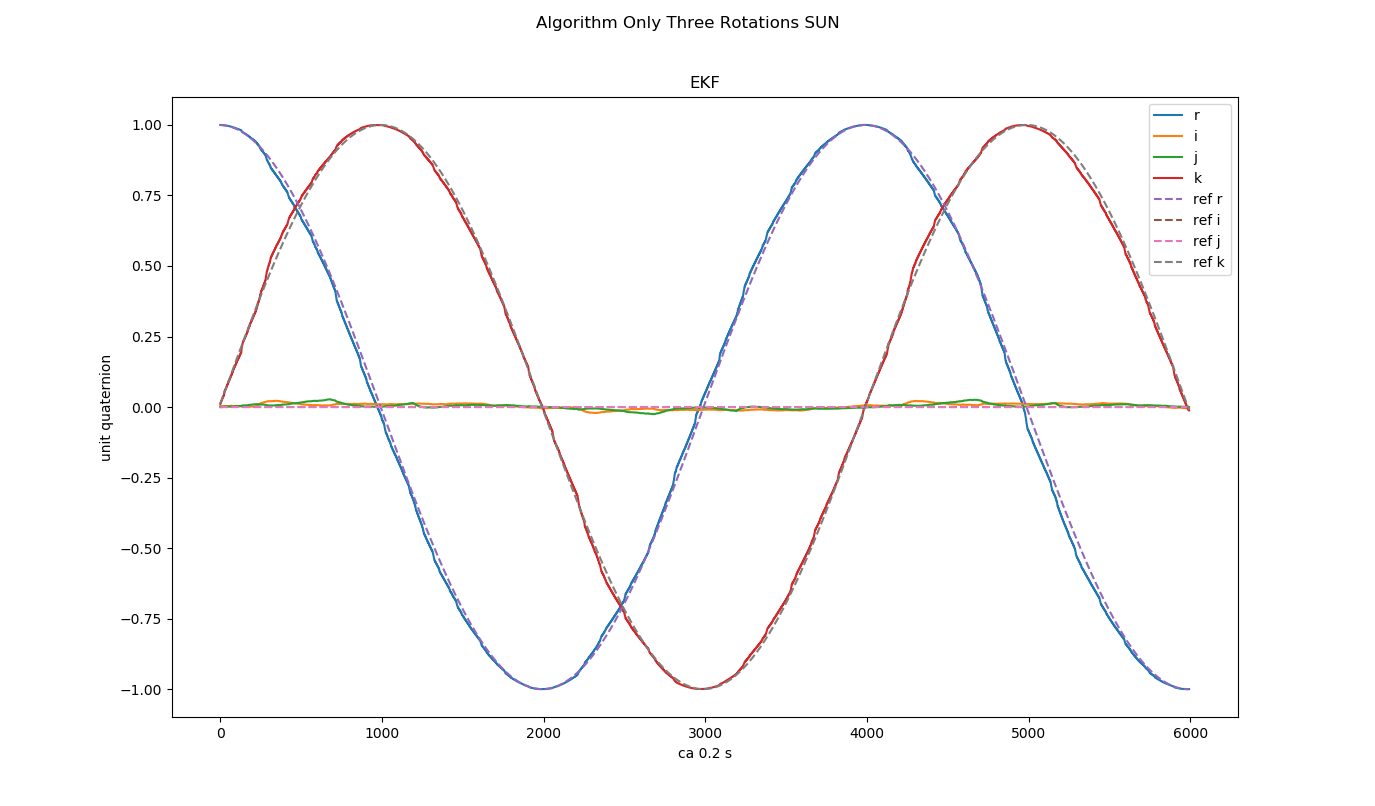
\includegraphics[width=1\columnwidth]{./Pictures/cdrRun3ThreeRotationsSun}
	\caption{Plot of recorded quaternion and reference quaternion for Algorithm only test using the PrintSat. Three rotations whit sun}
	\label{fig:cdr3RotSun}
\end{figure}               

\begin{figure}[tbp]
	\centering
	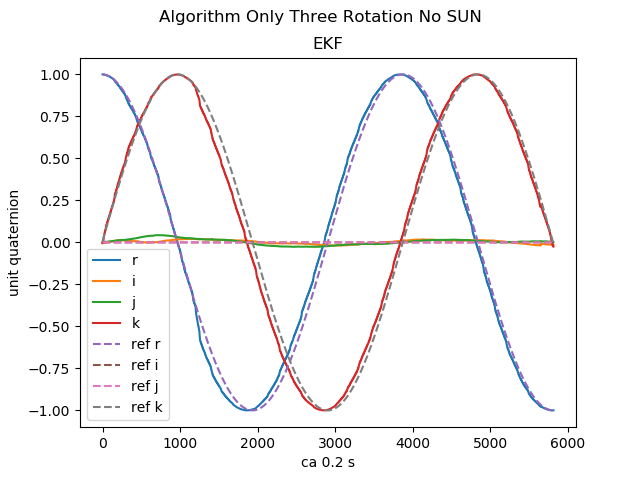
\includegraphics[width=1\columnwidth]{./Pictures/cdrRun3ThreeRotationsNoSun}
	\caption{Plot of recorded quaternion and reference quaternion for Algorithm only test using the PrintSat. Three rotations whit  no sun}
	\label{fig:cdr3RotNoSun}
\end{figure}

\subsection{PrintSat Outdoor Results}
When conducting the outdoor test there was no possibility of conducting tests whit rotations as there was problems getting the turntable to work whit batteries. A problem arises when there is no rotation. In \autoref{fig:OutdoorNoRotationSun} which is a test whit sun and no rotation it seems to be fine. The recorded quaternion is about [1 0 0 0] which is expected as the PrintSats body-fixed frame is aligned whit the lab frame. In \autoref{fig:OutdoorNoRotationNoSun} which is no sun and no rotation the EKF starts to struggle. From the results it seems like quaternions are converging towards the correct values, but the test is to short to say for sure what the quaternions are converging towards. Even if the quaternions are converging towards the right value it is way to slow. For the current implementation of the attitude controller this is not a  problem as it is a spinning controller, but one of the main reasons that the EKF is being implemented is to allow for the possibility to implement other types of controllers. One of this future controller could be a non spinning controller and the EKF should therefor be able to handle this scenario. Even if the problem does not affect the current design and is unlikely to come up in use it is a bug and before the root cause is discovered it is impossible to say what other side effects it might have.

\begin{figure}[tbp]
	\centering
	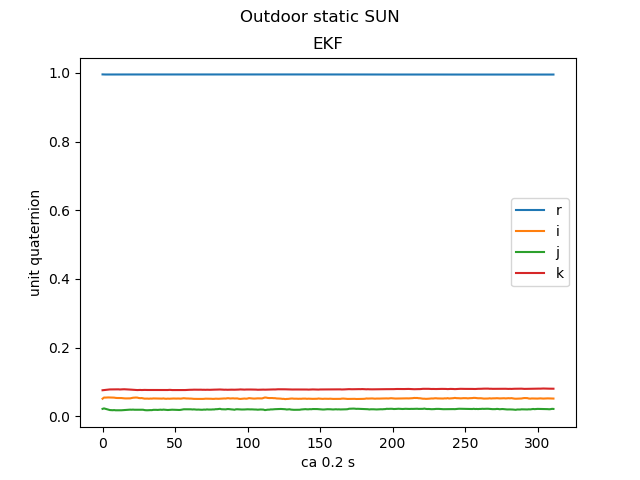
\includegraphics[width=0.6\columnwidth]{./Pictures/run3OutdoorStaticSUN}
	\caption{Plot of recorded quaternion quaternion for Outdoor test using the PrintSat. Static test whit sun}
	\label{fig:OutdoorNoRotationSun}
\end{figure}

\begin{figure}[tbp]
	\centering
	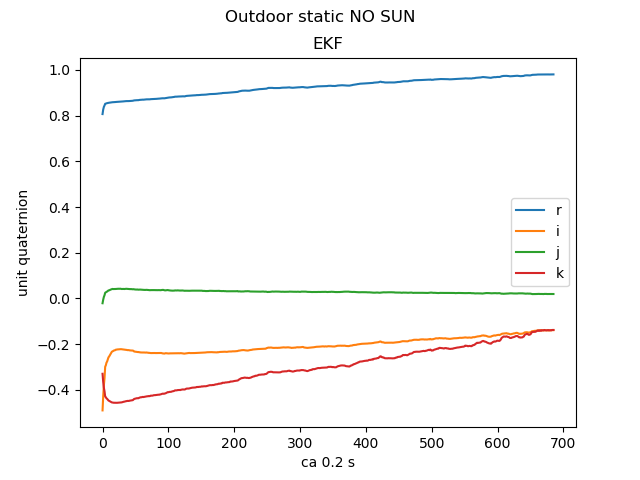
\includegraphics[width=0.6\columnwidth]{./Pictures/run3OutdoorStaticNOSUN}
	\caption{Plot of recorded quaternion for Outdoor test using the PrintSat. Static whit  no sun}
	\label{fig:OutdoorNoRotationNoSun}
\end{figure}         

Some effort have been put into trying to figure out why this happens. An initial theory was that it is due to the fact that the EKF is not initialized by the SVD and that it will converge to the right value give enough time. It is just so slow because the initial estimate is so far away from the correct estimate. The problem whit this theory is that the ADS seems to work when there is rotation and no sun. In this scenario there is also no SVD initialization, so it seems like the EKF works even whit out the SVD initialization. As a part of the future investigation a static Algorithm only test where conducted where the conditions where changed from sun to no sun before it was set back to sun. The results can be seen in \autoref{fig:cdrSunNoSunSun}. The results show that the quaternions stay constant even when there is sun if they have converged to the right values first. This at least indicates that the EKF does not diverge if the quaternions have already converge to the right value. For future investigation the problem have been recreated in simulations. This also indicates that the problem is a problem whit the algorithm it self and not the implementation on the satellite or any hardware related issues. 

\begin{figure}[tbp]
	\centering
	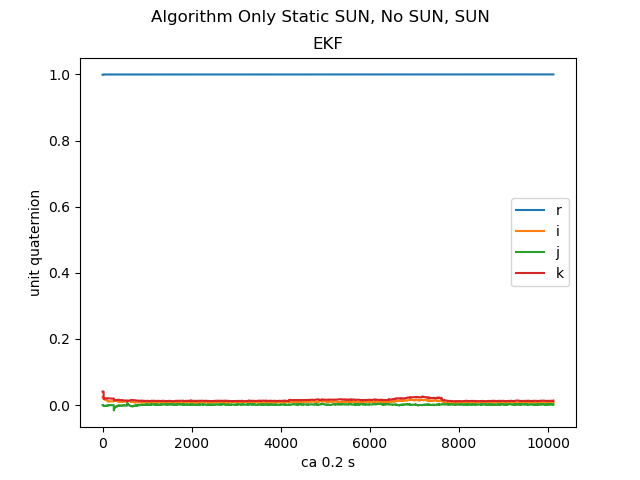
\includegraphics[width=0.6\columnwidth]{./Pictures/cdrRun1StaticSunEclipsSun}
	\caption{Plot of recorded quaternion for Algorithm only test test using the PrintSat. Static test where the condition are changed from sun to no sun and then back to sun. }
	\label{fig:cdrSunNoSunSun}
\end{figure} 

\subsection{PrintSat Reference Model Verification}
During the Outdoor test it is also possible to investigate how close the measurements are to there respective reference models. In \autoref{fig:magRef} the measured magnetometer data is plotted whit the reference magnetic vector from simulation and the one from reference vector calculated by the PrintSat. The simulated reference vector and the reference vector calculated by PrintSat are seemingly exactly the same, confirming that the reference vector calculated on the PrintSat is correct. There is some discrepancy between then measured vector and the reference vector, but overall it looks good. The main discrepancy is in the measurement of the z-axis. This also leads to a a difference between the lengths of the vectors. This error is not significant as when you normalize the vectors they become practically the same and the EKF uses the normalized vector. The error can also most likely be avoided by changing some of the parameters in the calibration procedure of the magnetometer resulting in an increase scaling of the z value to match the reference vector.           

\begin{figure}[tbp]
	\centering
	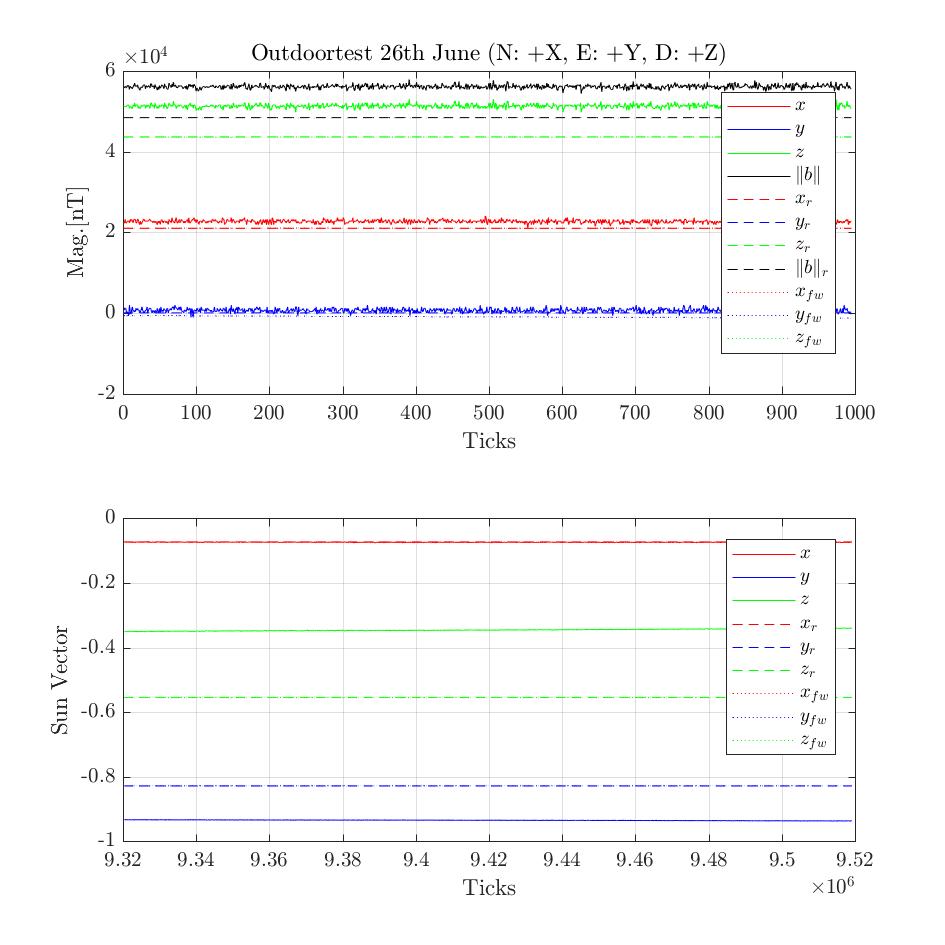
\includegraphics[width=0.8\columnwidth]{./Pictures/outdoor4}
	\caption{Plot of recorded magnetometer and sun sensor measurements plotted whit the simulated reference vectors and the reference vector calculated by the PrintSat. No lines subscript is sensor data, r subscript is simulated reference vector and subscript fw is reference vector from PrintSat}
	\label{fig:magRef}
\end{figure}

For the sun sensor the simulated and calculated reference vector are exactly the same meaning that the reference vector for the sun position is also correctly calculated on the PrintSat. The measured sun vector is quit far away from the reference vector. The reason for this is still not clear. All functionality test of the sun sensor indicates that they are working properly. A new method for calibrating the sun sensor where developed by another member of the ADCS team during this period. Despite using the new calibration method the results are still pore. A possible explanation could be that the error comes from the transformation of the measurements in sensor frame to the body-fixed frame. The transformation is assumed to be a \SI{90}{\degree} rotation around the axis of the body-fixed frame. This comes from the assumption that the side panels are parallel to the axis of the body-fixed frame. This assumption is not true on the PrintSat as the structure is not that rigged. The results also indicates that the EKF is capable to function even if the sun sensor measurements are not that good.                      

\section{Flight Model}
The test whit the FM where limited in scope and mostly to verify that the same behavior that is seen on the PrintSat can be seen on the FM. There results from two test shown in \autoref{fig:FMcdrTwoRotSun} and \autoref{fig:FMcdrTwoRotNoSun} show that the results are somewhat consistent whit the PrintSat. The overall trend in both is that ADS is preforming reasonably well and the estimated quaternions are able to follow the reference quaternions reasonably well. In \autoref{fig:FMcdrTwoRotSun} the preference is a lot worse than on the PrintSat equivalent test seen in \autoref{fig:cdr3RotSun}. There are this seemingly periodic shifts in the estimated quaternion that was not so viable on the PrintSat. This seems to come from spikes in the sun sensor measurements as you can see in the bottom plot of \autoref{fig:FMcdrTwoRotSun} there is a shift in the estimated quaternion when ever there are spikes in the sun sensor measurement. The spikes in the sun sensor measurements seem to come from when there is a switch in which sun sensor that is being used. The switching comes from  a new side panel facing the sun. The reason why the spikes in sun sensor measurements are only on the FM and not on the PrintSat is still under investigation, but the working theory is that the spikes comes from the environment. As the FM test was conducted in the integration room that is not completely dark while the PrintSat test where done in a complete dark room. The main reason environmental factors are consider the reason is that under all functional test of the FM sun sensors the sun sensors have preformed as expected and similar to the results to the sun sensor of the PrintSat.   

The one shift that can be seen in \autoref{fig:FMcdrTwoRotNoSun} also comes from when the natural light in the integration room was accepted as a valid sun sensor measurement and therefore used in the EKF cosing the shift. One thing that is interesting to note is that the quaternion does not converge back to the correct estimate but instead follows the reference quaternion whit a constant error.

\begin{figure}[tbp]
	\centering
	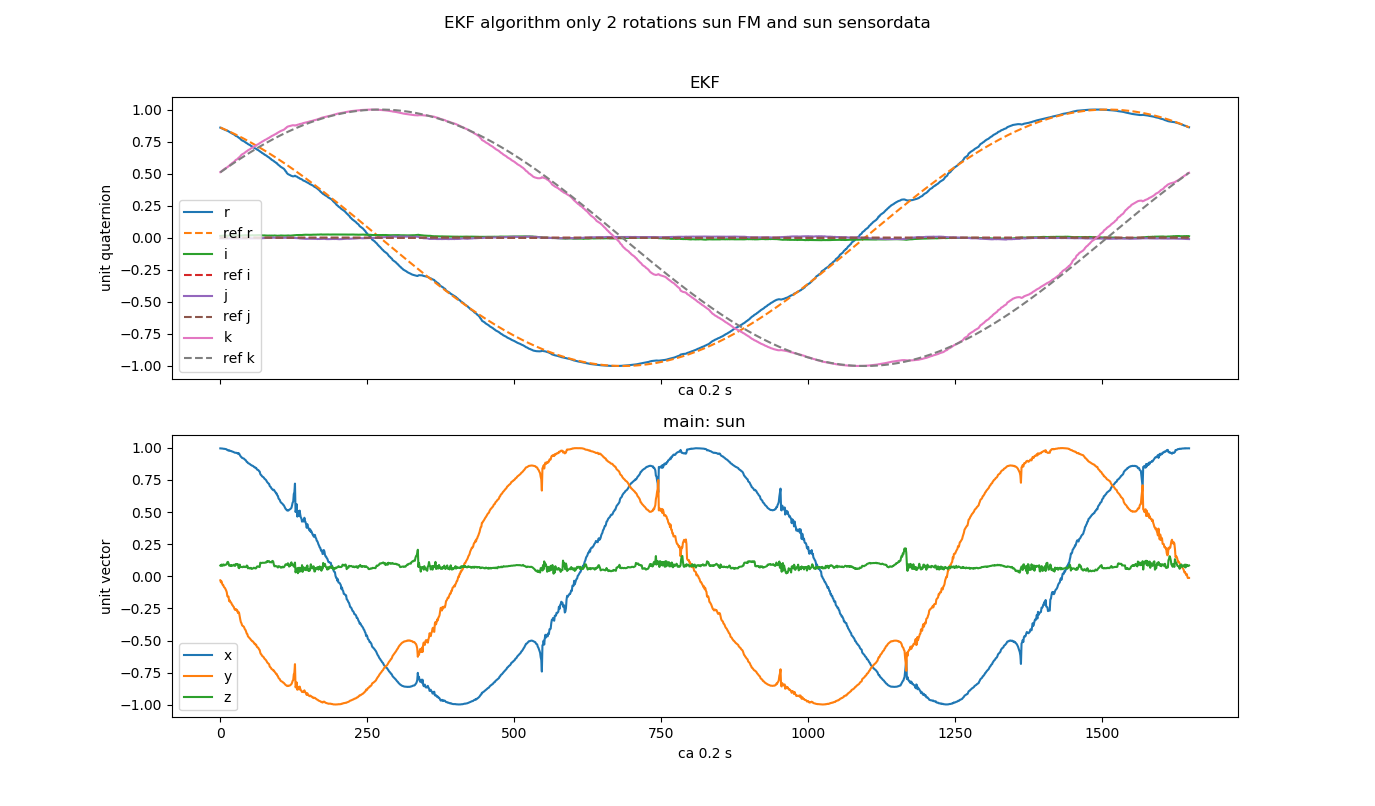
\includegraphics[width=1\columnwidth]{./Pictures/test1EKFandSUN}
	\caption{Plot of recorded quaternion for Algorithm only test test using the FM and the recorded sun sensor measurements. The FM is turned two time on the turntable.}
	\label{fig:FMcdrTwoRotSun}
\end{figure}

\begin{figure}[tbp]
	\centering
	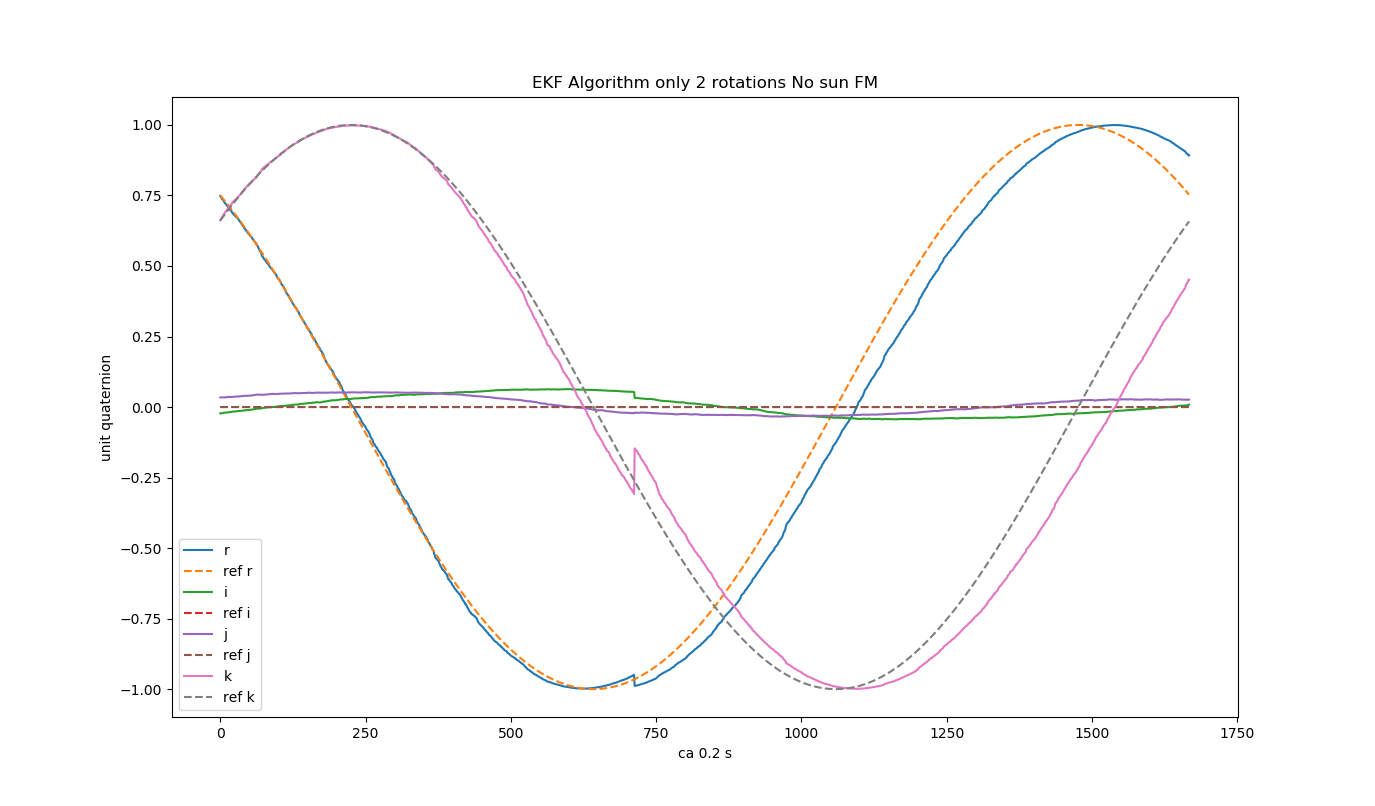
\includegraphics[width=1\columnwidth]{./Pictures/EKF_Algorithm_only_2_rotations_No_sun_FM}
	\caption{Plot of recorded quaternion for Algorithm only test using the FM. The FM is turned two times on the turntable.}
	\label{fig:FMcdrTwoRotNoSun}
\end{figure}   



%\chapter{Einleitung}
%\chapter{Introduction}
%\chapter{R�sum� und Ausblick}
\chapter{Conclusion}
\label{sec-conclusion}
The MOVE-II CubeSat to project is a project aiming to an educational platform and give students relevant experience in the space industry. To accomplice this a CubeSat has been built primarily by students. The satellite is expected to be launched sometime in October. The payload of the satellite is experimental solar cells. To conduct recordings of the efficacy of the solar cell when they are in space it is required that they face the sun. To accomplish this an ADCS was needed. As part of the ADCS an attitude determination system based around an extended Kalman filter was design. This ADS was not sufficiently tested before the launch software was locked, but the software can still be updated when the satellite is in space. Resent simulations show that the current controller is not very power efficient and there is a deicer to do an update of the controller. For the new controller the attitude needs to be determined. So it is therefore important to properly test and verify of current ADS to facilitate for this new controller. 

Two different methods for testing the ADS was developed and used. One was a simpler method testing only the algorithm is self and not the full system called Algorithm only. The other method tested almost the full system and was called Outdoor. Bot test where able to give valuable information about the functionality of the ADS. The main findings show that the ADS works nicely under good conditions. That is in the sun and whit a spinning satellite. The test also revealed some weaknesses of the ADS. Namely that the ADS does not work whit a stationary satellite and no sun. It also shows that the estimated attitude is very vulnerable to disturbances on the sun sensor. The reason for why it does not work whit no sun and a static satellite is still unknown. It also showed that the calculated reference models are correct.             

\chapter{Outlook}
\label{sec-outlook}
Moving forward there are two main areas that should be looked at. The first is investigating some of the anomalies discovered by the test. The main anomaly that needs to be future investigated is why the ADS does not work with a stationary satellite and no sun. As the anomaly is reproducible in simulations it seems like continuing to investigate the problem in the simulation environment is the beater option. As the simulation environment is a lot easier and faster to work whit when you are doing debugging. Once the problem is discovered and solved one could go back to the hardware test for verification. 

Smaller issues to be resolved are solving the discrepancy between the reference model and the measurements. For the magnetometer is seems like changing the parameters for the calibrations method to get higher scaling is the way to proceed. For the sun sensor the way is a bit more unclear and a lot more investigation is needed. Looking into the transformation between sensor and body-fixed frame might be a starting point. 

The second are is development of the so called UWE-3 approach. The UWE-3 approach as the Outdoor test has the advantage that they test almost the entire system. The advantage the UWE-3 approach has over the Outdoor test is that is can be conducted using a permanent setup inside. This allows for a more efficient setup as you do not have to bring inn all the equipment outside all the time. It also has the advantage that it is not dependent on the sun. Meaning test could be conducted all year around. To develop the approach a suitable light source most be acquired and the function to find the correct time based on the position of the light source most be developed.                     
%
%
% ENDE EINBINDUNG BENUTZERDATEIEN
% **************************************************************
% **************************************************************

%
%
%  ANHANG
% +++++++++++++++++++++++++++++++++++++++++++++++
% Der Anhang wird durch die Umgebung appendix vom
% Rest der Arbeit abgegrenzt und hat eine eigene
% Darstellung der Überschriften und Kopfzeilen.
% Binden Sie ihre Anhangskapitel in der Datei Anhang.tex ein.
%
%\begin{appendix}
%    \input{TexFiles/Appendix}
%\end{appendix}
%
% ENDE ANHANG
%
% FORMELZEICHEN UND EINHEITEN
% +++++++++++++++++++++++++++++++++++++++++++++++
%
%\def\chaptermark#1{}
%\mark{{}{}}   % Initialisierung der Markierungen (wirkt wie ein Reset)
%\input{TexFiles/List-of-Symbols}
%
%\input{TexFiles/List-of-Abbreviations}%
%
% VERZEICHNIS DER VORKOMMENDEN ABBILDUNGEN
% +++++++++++++++++++++++++++++++++++++++++++++++
%\listoffigures
%
%
% VERZEICHNIS DER VORKOMMENDEN TABELLEN
% +++++++++++++++++++++++++++++++++++++++++++++++
%\listoftables
%
%
% LITERATURVERZEICHNIS
% +++++++++++++++++++++++++++++++++++++++++++++++
% Wichtig: Dieses ist immer einspaltig ausgeführt.
\bibliographystyle{acm}
\bibliography{DiplomaThesis-Literature}
%
%
%
% INDEX
% +++++++++++++++++++++++++++++++++++++++++++++++
% Hierzu muss an entsprechender Stelle im Text mit
% \index{Bezeichnung} eine Referenz erzeugt werden
%
% **manual**
%\printindex
%
%
%\cite{*}
\end{document}
% DOKUMENT ENDE
% ----------------------------------------------------------------

